%% 
%% Copyright 2019-2021 Elsevier Ltd
%% 
%% This file is part of the 'CAS Bundle'.
%% --------------------------------------
%% 
%% It may be distributed under the conditions of the LaTeX Project Public
%% License,  either version 1.2 of this license or (at your option) any
%% later version.  The latest version of this license is in
%%    http://www.latex-project.org/lppl.txt
%% and version 1.2 or later is part of all distributions of LaTeX
%% version 1999/12/01 or later.
%% 
%% The list of all files belonging to the 'CAS Bundle' is
%% given in the file `manifest.txt'.
%% 
%% Template article for cas-sc documentclass for 
%% single column output.

\documentclass[a4paper, fleqn]{cas-sc}

% If the frontmatter runs over more than one page
% use the longmktitle option.

%\documentclass[a4paper, fleqn, longmktitle]{cas-sc}

\usepackage[numbers]{natbib}
%\usepackage[authoryear]{natbib}
%\usepackage[authoryear, longnamesfirst]{natbib}
\usepackage{graphicx}
\usepackage{multirow}
\usepackage[normalem]{ulem}
\useunder{\uline}{\ul}{}
\usepackage{lscape}
\usepackage{longtable}
\usepackage{booktabs, tabularx}
\usepackage{float}
\usepackage{subfigure}
\usepackage[section]{placeins}


%%%Author macros
\def\tsc#1{\csdef{#1}{\textsc{\lowercase{#1}}\xspace}}
\tsc{WGM}
\tsc{QE}
%%%

% Uncomment and use as if needed
%\newtheorem{theorem}{Theorem}
%\newtheorem{lemma}[theorem]{Lemma}
%\newdefinition{rmk}{Remark}
%\newproof{pf}{Proof}
%\newproof{pot}{Proof of Theorem \ref{thm}}

\begin{document}
\let\WriteBookmarks\relax
\def\floatpagepagefraction{1}
\def\textpagefraction{.001}

% Short title
\shorttitle{A novel Reductive Bias and Hybrid GRU-CNN (RB-GRU-CNN) Model for Prediction of PTB Diagnostic ECG Time Series Data.}    

% Short author
\shortauthors{S. Khan}  

% Main title of the paper
\title [mode = title]{A novel Reductive bias and Hybrid GRU-CNN (RB-GRU-CNN) model for prediction of PTB diagnostic ECG Time Series data.}  


\begin{comment}
% Title footnote mark
% eg: \tnotemark[1]
\tnotemark[<tnote number>] 

% Title footnote 1.
% eg: \tnotetext[1]{Title footnote text}
\tnotetext[<tnote number>]{<tnote text>} 

% First author
%
% Options: Use if required
% eg: \author[1, 3]{Author Name}[type=editor, 
%       style=chinese, 
%       auid=000, 
%       bioid=1, 
%       prefix=Sir, 
%       orcid=0000-0000-0000-0000, 
%       facebook=<facebook id>, 
%       twitter=<twitter id>, 
%       linkedin=<linkedin id>, 
%       gplus=<gplus id>]

\author[<aff no>]{Subham Kumar}[<options>]

% Corresponding author indication
\cormark[<corr mark no>]

% Footnote of the first author
\fnmark[<footnote mark no>]

% Email id of the first author
\ead{subh700454@gmail.com}

% URL of the first author
\ead[url]{<URL>}

% Credit authorship
% eg: \credit{Conceptualization of this study,  Methodology,  Software}
\credit{<Credit authorship details>}

% Address/affiliation
\affiliation[<aff no>]{organization={}, 
            addressline={},  
            city={}, 
%          citysep={},  % Uncomment if no comma needed between city and postcode
            postcode={},  
            state={}, 
            country={}}

\author[<aff no>]{<author name>}[<options>]

% Footnote of the second author
\fnmark[2]

% Email id of the second author
\ead{}

% URL of the second author
\ead[url]{}

% Credit authorship
\credit{}

% Address/affiliation
\affiliation[<aff no>]{organization={}, 
            addressline={},  
            city={}, 
%          citysep={},  % Uncomment if no comma needed between city and postcode
            postcode={},  
            state={}, 
            country={}}

% Corresponding author text
\cortext[1]{Corresponding author}

% Footnote text
\fntext[1]{}

% For a title note without a number/mark
%\nonumnote{}


\end{comment}



% Here goes the abstract
\begin{abstract}
  Time series analysis plays a vital role in medical sciences. It is been of great importance lately to understand the dynamics of data to predict and account for the state of survivability in patients with various conditions. The objective of our work is to understad time series ECG data of patients with certain heart conditions and checking their ECG  prediction error on multiple performance metrics based on Deep learning(DL) models. An array of multichannel ECG recordings were obtained from patients with a variety of cardiac conditions. As the heart's electrical activity over time is recorded,  we gain valuable insight into patient's health. A time series analysis is performed on five patient records since it is a very large database. This is accomplished using advanced DL algorithms significantly used these days for time series analysis (CNN, RNN, LSTM, GRU, BiLSTM). Our Proposed model has a significantly better performance over RMSE,  MSE,  MAE and MAPE upon traditional DL Models. As a result of these findings, The author has demonstrated effectiveness of the proposed approach in predicting the progression of cardiac abnormalities. Health professionals can use these models to make informed decisions and provide timely interventions for patients with cardiac conditions. This study showcases the significance of time series analysis techniques in improving diagnostic capabilities and enhancing patient care in the field of cardiology.
\end{abstract}

% Use if graphical abstract is present
%\begin{graphicalabstract}
%\includegraphics{}
%\end{graphicalabstract}

 

% Keywords
% Each keyword is seperated by \sep
\begin{keywords}
  Time series analysis \sep ECG \sep Electrocardiogram \sep PTB Diagnostic ECG Database \sep Deep Learning\sep Cardiac abnormalities\sep Healthcare \sep Diagnostics\sep Anomaly detection \sep
\end{keywords}

\maketitle

% Main text
\section{Introduction}
The ECG is widely used as a non-invasive diagnostic tool,  revealing useful information about the electrical activity of the heart. It's possible for healthcare professionals to learn a great deal about the cardiac health of individuals by analysing the temporal patterns and characteristics of ECG signals. Signal interpretation is a time-taking and intricate task,  therefore there is a chance of subjective ambiguity and human mistake in the analysis process,  even for experts who have spent years learning. As a result,  it is essential to prioritise computer-aided method for research  and development in time series analysis.  Computer-assisted analysis can analyse ECG signals more precisely and promptly,  with no differences caused by inter-operators or operator-specific differences \cite{liu2021deep}. Since ECG is a time series data,  it can be observed by work of \cite{dudukcu2023temporal} that hybrid deep neural network approaches outperform single deep neural network methods in dealing with time series prediction. The proposed model achieved an average RMSE of 0.0022 for chaotic data whereas 0.0082 for ECG Arrythmia dataset. Since, multiple model's integration outperform single traditionl model.   \cite{zhang2007neural} stated the proposed strategy consistently outperforms the single modelling approach for a range of time series processes. The analysis of electrocardiograms (ECGs) can be one of the areas in which it can be used extensively. PTB Diagnostic ECG dataset can be a valuable resource in this regard. A vast collection of ECG recordings is found in the PTB dataset,  including recordings from patients with a variety of cardiac conditions. Recordings capture the electrical activity of the heart over time,  creating a time series data structure. With the help of time series analysis techniques,  researchers and medical professionals can uncover hidden patterns,  identify abnormalities,  and develop predictive models for accurate cardiac diagnosis.
\par The use of automation in the field of cardiac illness diagnosis may aid in the accurate and timely examination of heart problems \cite{rahul2020exploratory}. The primary purpose of time series analysis of the PTB Diagnostic ECG dataset is to extract meaningful insights from the temporal dynamics of the ECG signals. Data preprocessing,  feature extraction,  anomaly detection,  and classification are some of the research areas widely performed in this domain. It is possible to detect specific ECG patterns associated with different cardiac conditions using advanced algorithms and statistical methods. This allows accurate diagnosis and timely treatment of the condition. ECG time series analysis as a means of improving cardiac diagnostics has the potential to revolutionise this field. In addition to enhancing detection accuracy,  it can also assist in the early detection of cardiovascular diseases,  and assist in the planning and implementation of personalised treatment plans. \par With our proposed model, It is possible,  too,  to use the knowledge gained from this analysis to develop automated ECG analysis systems,  empowering healthcare professionals with efficient tools for cardiac assessment. Using time series analysis techniques,  author aim to reveal the diagnostic potential of the PTB Diagnostic ECG dataset. To advance cardiac healthcare,  also seek to provide valuable insight into the temporal dynamics of ECG signals,  their association with cardiac conditions,  and their application to Cardiological treatment. (Note: The PTB Diagnostic ECG dataset refers to the publicly available dataset from the Physikalisch-Technische Bundesanstalt (PTB),  which contains ECG recordings of patients with different cardiac conditions).

\section{Related work}
ECG data indicates the cardiac muscle's electrical activity as detected by electrodes put on the skin. The ECG is useful in detecting normal and acute coronary syndrome,  irregular heart rhythms,  and additional cardiac and noncardiac abnormalities. Researchers have also employed the ECG to analyse sleep,  emotions,  and stress. Several studies have found that physicians are frequently inept at reading ECGs in clinical practise \cite{bond2012effects}. Therefore a major number of academics have employed machine learning to see if AI can help enhance ECG interpretation and clinical decision making \cite{rjoob2022machine}. With DL,  we are attempting to introduce this approach of study. The main justification for employing DL The advantage of using it for ECG interpretation is that it may potentially analyse intricacies in ECG signals that clinicians do not normally investigate. One of the major reason behind using DL in this work is large number of data points. Since,  when the dataset is huge, DL algorithms can outperform other techniques \cite{purushotham2018benchmarking}. Also a vast majority of researches from air pollution \cite{kumar2022deep} to Medicine,  Automobiles \cite{naqvi2018deep},  Sales\cite{kaneko2016deep},  etc are being conducted in DL with promising results and future scopes.  Because of their capacity to extract features automatically,  deep neural networks have found remarkable success in a wide range of healthcare concerns. \cite{midani2023deeparr} gave a DeepArr model which provides an accuracy of 99.46\% on MIT-BIH Arrythmia dataset. A gated recurrent unit (GRU) was utilised to learn the intrinsic time features of SHM time series in order to extract the temporal feature vectors \cite{li2022hybrid}. Their CNN-GRU Heave attained RMSE of 1.3655 whereas Pitch gave an RMSE of 0.0350 . 
\par The objective of the \cite{prakarsha2022time} was to find a method for forecasting signals in time series with high accuracy using neural networks and beat the conventional method of adaptive filters in this regard. They claimed their approach may even eliminate the need to de-noise the signal before analysis,  as ANNs outperformed LMS filters by giving a forecasting accuracy of 95.72\%. Novel filtering method like Butterworth filtering is introduced in the studies of ECG. However,  the main purpose is to perform feature extraction which is done by DL models itself. When dealing with univariate time series,  traditional discriminant analysis techniques may be applied to leverage time series features such as autocorrelations,  periodogram coefficients,  wavelet features,  and so on. Several writers have proposed univariate time series discriminant analysis \cite{maharaj2007discrimination}. \cite{hammad2021automated} found that using a single feature resulted in poor performance when compared to combination of features. Also they recommended to use wavelet transform with CNN which can ensure a good accuracy even for small datasets. 
\par In recent years,  traditional ML algorithms have acquired unsatisfactory performance as a result of methods known as handmade approaches. Handcrafted feature engineering, in which a data scientist selects a set of variables with predictive powers,  is not required for DL,  as DL can conduct this filtering automatically. Experiments were carried out on CNN,  RNN,  GRU,  LSTM,  and BiLSTM, and a hybrid model combining 1D-CNN and GRU is created. CNNs are also utilised for one-dimensional data processing,  such as time series analysis \cite{sajjad2020novel} and our dataset is univariate and one-dimensional too. \par A feed forward neural network with a hierarchical structure is referred to as a convolutional neural network \cite{chua1998cnn}. CNN employs the weight-sharing principle as stated by \cite{qiu2018variety} which performs well on non-linear challenges such as time series prediction. CNN has grown popular in ECG feature extraction due to its capacity to learn favourable features from ECG input data in order to recognise patterns\cite{wang2023inter}. Because each neuron's layer in GRU effects the output at subsequent moments,  it can be utilised to characterise time series and handle gradient disappearance and gradient explosion difficulties in long sequence training \cite{dey2017gate}. Furthermore,  the GRU has two gating units that regulate how new information is integrated with old information and how much of the previous information is retained to calculate the new state,  resulting in significantly reduced calculation time throughout the feature extraction process \cite{yao2021interpretation}. The potential difference between electrodes placed on distinct parts of the body tissue is measured and recorded with an electrocardiograph or a vector electrocardiograph to produce an ECG. The aberrant activity of the heartbeat can thus be demonstrated\cite{liu2021deep}. The ECG can predict coronary heart disease. There have been studies that show ECG is useful in terms of predicting both short- and long-term results
. For individuals suffering from myocardial infarction,  for example,  the earlier the irregular cardiac rhythm is recognised,  the better the chances of avoiding life-threatening complications and recovering \cite{pollard2000acute}. Because ECG signals have considerable noise and complexity,  identifying specific disorders can be time-consuming and labor-intensive. Another issue is individual variation \cite{de2011weighted}. According to the researchers Because many signs and markers of cardiovascular disease can be found in physiological data other than ECG,  vital data such as respiratory rate and blood pressure can be utilised in conjunction with ECG to aid in diagnosis.
\cite{xu2018raim}. Occurance of sleep apnea can be diagnosed with DL forecasting of single lead ECG. A forecasting accuracy of 94.95\% is obtained using deep recurrent neural network \cite{bahrami2022deep}. Mainly Classification tasks are being performed on ECG dataset \cite{strodthoff2020deep}. Classifications involving wavelet transforms and encoding decoding\cite{mewada20232d}. Algorithms in DL are referred to as a 'black box',  which means there is no transparency and,  as a result,  no explanation is available to the users to provide some rationale as to what is going on inside the black box or why the DL algorithm produces an outcome in particular \cite{von2021transparency}. CNN-BiLSTM achieved an accuracy of 95\% on diagnosing atrial fibrillation\cite{aldughayfiq2023deep}. An avaerage RMSE of 0.082 is achieved by \cite{yoo2023restoration} after restoring missing signals using ensemble model. A comprehensive study can be found in the review literature \cite{musa2023systematic}


\section{Dataset and Exploratory Analysis}
 
\textbf({Exploratory Data Analysis(EDA)}): Dataset is taken from Physionet ATM. The PTB Diagnostic ECG Database \href{https://physionet.org/content/ptbdb/1.0.0}{(https://physionet.org/content/ptbdb/1.0.0)} consist of ECG reports of 294 subjects,  which includes healthy subjects as well as patients with various heart disease conditions. All datasets contain 10000 samples each. Data points are distributed in a cycle of 10 seconds each. Sampling rate is set to 1000. Single lead ECG data (lead-{II}) of five patients has been taken since PTB diagnostic ECG database is very large database with 290 subjects and it was not possible to study all individually hence we took five records with different distributions. Since majority among the researches evaluated the effectiveness of computer-aided methods on (lead-II) ECG,  which is taken in previous studies \cite{liu2021deep}. This is how they look Figure  \ref{Fig:1}. Here (P1, P2, P3, P4 and P5) are patient's recorded ECG :
\begin{figure*}[ht!]
    \centering
     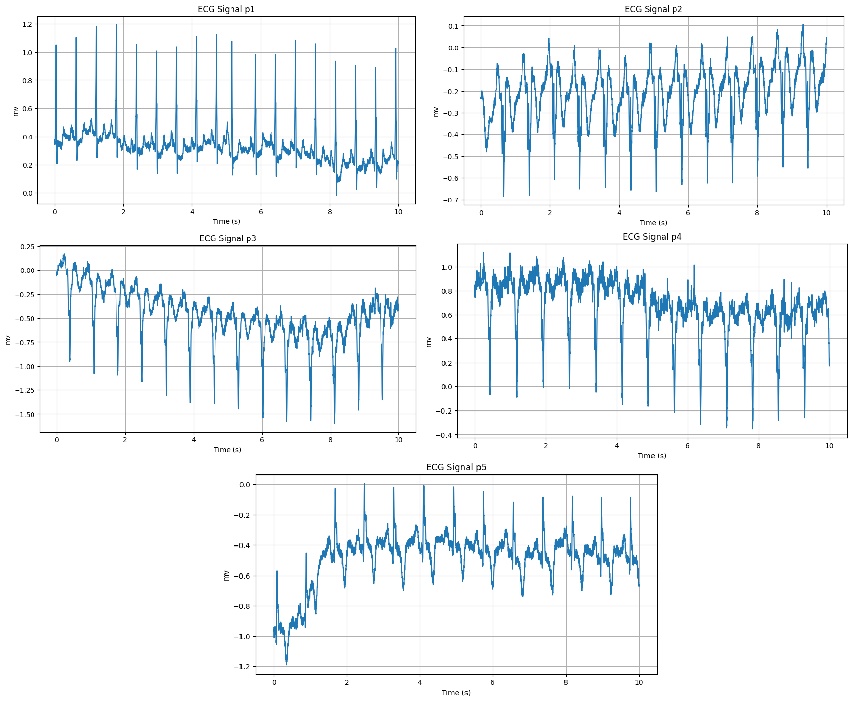
\includegraphics[scale=1]{edadrawio.pdf}
     \caption{Patient's(P1,  P2,  P3,  P4 and P5) ECG Plot}
     \label{Fig:1}
   \end{figure*}
\begin{figure*}[h!]
  \centering
   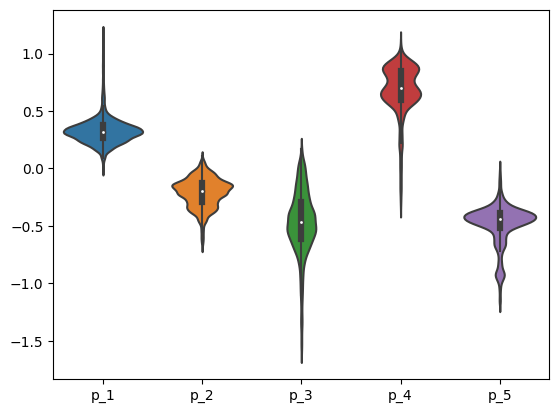
\includegraphics[scale=.5]{violin_plot_5_patients.png}
  \caption{Dataset distribution using violin plot}
   \label{Fig:2}
\end{figure*}

 
   \begin{figure*}[h!]
    \centering
     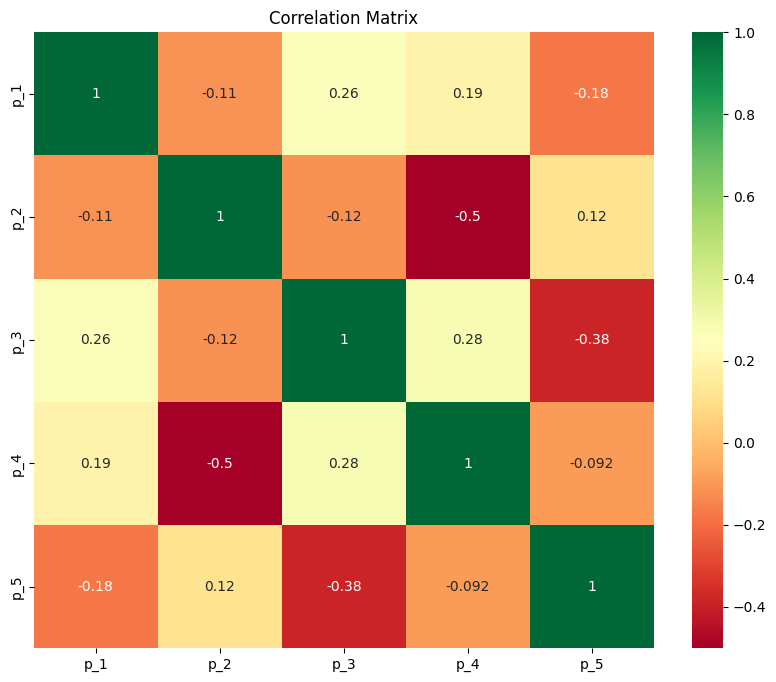
\includegraphics[scale=.42]{correlation_matrix_5_patients.png}
     \caption{Dataset's correlation matrix} 
     \label{Fig:3}
    \end{figure*} 

   \begin{figure*}[h!]
    \centering
     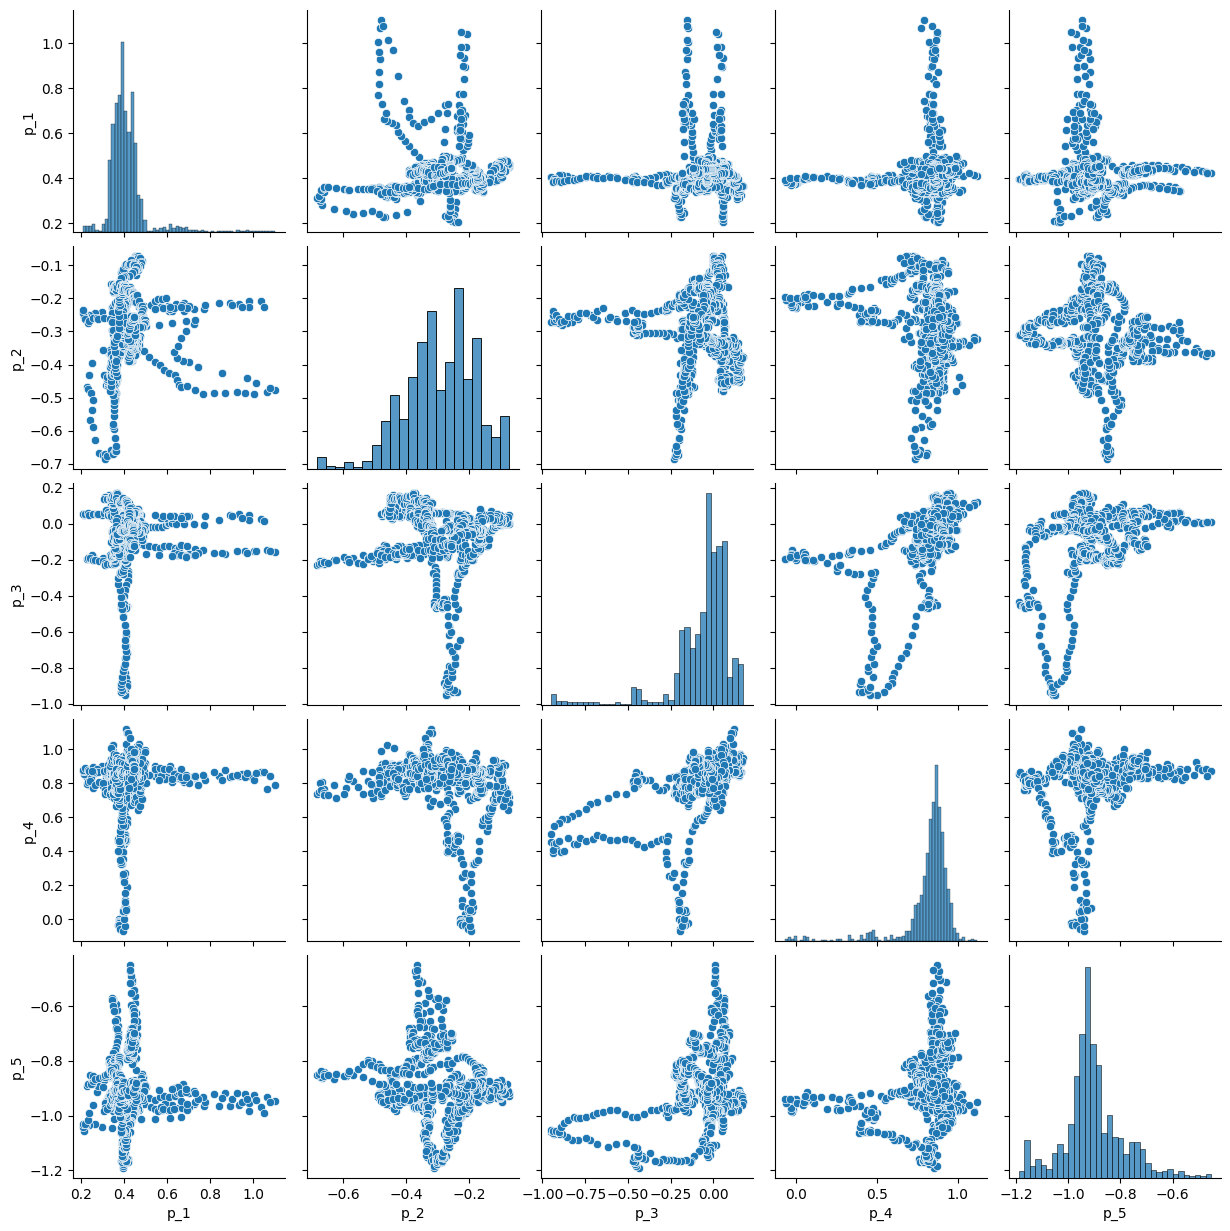
\includegraphics[scale=.52]{pair_plot.png}
     \caption{Patient's dataset distribution pair-plot}
    \label{Fig:4}
   \end{figure*}
  

 
 The plot has been drawn to look into distribution of our dataset With violin plot Figure  \ref{Fig:2} it can be understood whether the values are clustered around the median. Additionally,  it can be understood if the dataset values exhibit excessive clustering with an absence of values in the middle range. The Heatmap Figure  \ref{Fig:3} is representing correlation between the chosen datasets,  as it can be seen datasets with high collinearity are selected for studies. With pairplot Figure  \ref{Fig:4} pairwise relationship between datasets can be seen since it plots multiple pairwise bivariate distributions. The diagonal plots are univariate plots, and they show the relationship for the (n,  2) variable combination in a Dataframe as a matrix of plots.
Also  For time series analysis and dataset understanding,  statistical measures are used in conjunction with exploratory data analysis.
 
 
 
 
 \section{Proposed Methodology}
 
 
 \subsection{Proposed 1: Hybrid GRU-CNN Model}
 
 
 An end-to-end DL paradigm is used,  allowing for automated ECG analysis.  GRU addresses problems with long sequences with widely separated features. GRU makes the final choice on how much of the past should be remembered and how much should be forgotten. The GRU cell receives two inputs: the previous concealed state and the current timestamp. These are combined and passed through the update and reset gates by the cell. To predict the output in the current timestep,  the hidden state must be passed via a thick layer with an activation function. As a result,  a new hidden state is obtained,  which is then passed on to the following time step. The update gate selects which current GRU cell will send data to the next GRU cell. It aids in remembering the most crucial facts. Figure \ref{Fig:5} is our proposed framework:



    \begin{figure}
      \centering
      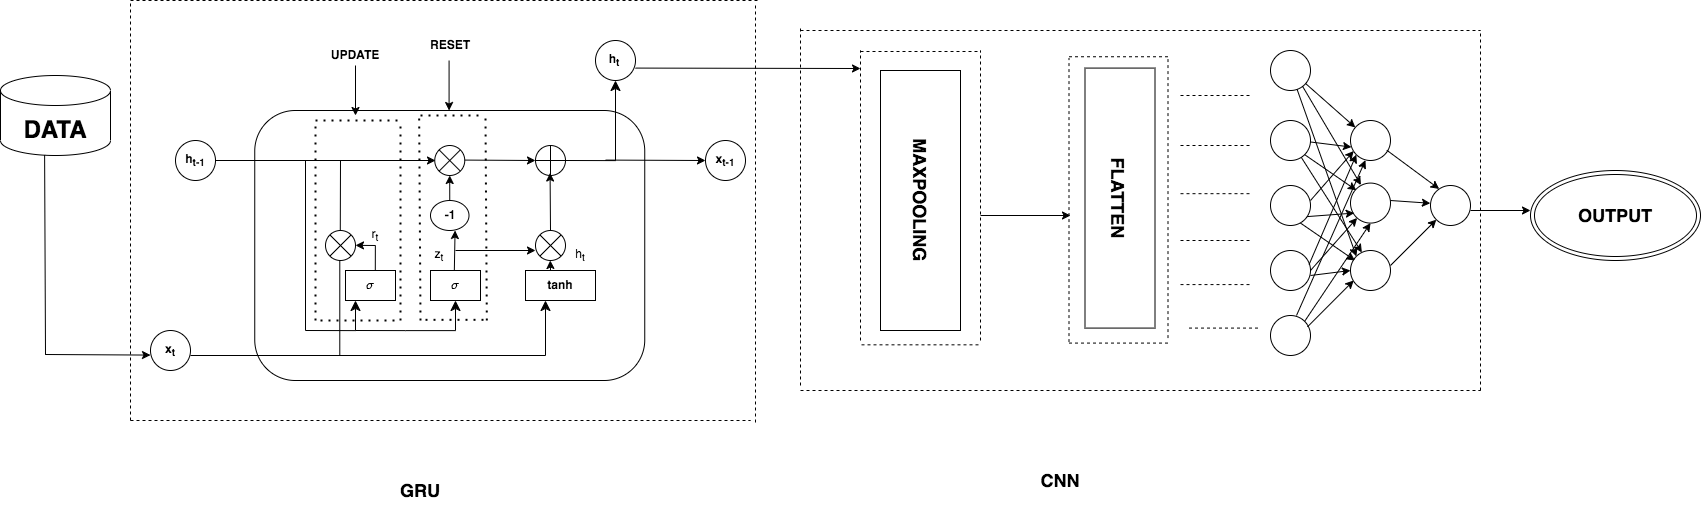
\includegraphics[scale= 0.25]{architecturepro1.png}
      \caption{Proposed hybrid GRU-CNN model framework}
      \label{Fig:5}
    \end{figure}



 Let our timeseries data be denoted as, 
 \begin{equation}
  X = [ x_1,  x_2,  x_3.... x_m]
 \end{equation}

where,   $x_t \in X$ and $[t = 1, 2, 3...m]$ ,  $t \in Z^+$ . The update gate's inputs are the hidden layer from the previous timestep $(h_{t-1})$ and the current input $( x_t )$. Both have related weights that are learned during the training phase. Let us say that the weights associated with $(h_{t-1})$ is $( U_z )$ and that of $( x_t )$ is $( W_z )$. The output of the update gate $( Z_t )$ is given by, 

\begin{equation}
  z_t = \sigma(W_z x_t + U_z h_{t-1})
\end{equation}
A reset gate identifies unnecessary information and decides what information to remove from the GRU network; in other words,  it decides what information to delete at a specific timestamp. The input to the reset gate is the hidden layer at the previous timestep $(h_{t-1})$ and the current input $( x_t )$ 
Both have related weights that are learned during the training phase.  Let us say that the weights associated with $(h_{t-1})$ is $(U_r)$ and that of  $( x_t )$ is $(W_r)$.  The output of the update gate $( r_t )$ is given by, 

\begin{equation}
  r_t = \sigma(W_r x_t + U_r h_{t-1})
\end{equation}

GRU networks interpret sequential data,  such as time series or plain language,  by avoiding the hidden state from one time step to the next. The hidden state is a vector that contains information from previous time steps that are relevant to the current time step. The primary principle behind a GRU is to let the network decide which information from the previous time step is relevant to the current time step and which may be ignored.


The reset gate is used to calculate a candidate's hidden state. This is utilised to determine the information that has been stored in the past. This is sometimes referred to as the memory component in a GRU cell. It is calculated as follows, 
\begin{equation}
  \tilde{h}_t = \tanh(W_{x_{t}} + r_t \odot U_{h_{t-1}})
\end{equation}

Here,  $W_{x_{t}}$ : Weight associated with the current input,  $r_t$ : Output of the reset gate,  $U_{h_{t-1}}$ : Weight associated with the hidden layer of the previous timestep,  $\tilde{h}_t$ : Candidate hidden state.



The new hidden state is calculated using the following formula,  which is dependent on the update gate and candidate hidden state.
\begin{equation}
  {h}_t = ( z_t \odot h_{t-1} + (1- z_t)\odot \tilde{h}_t)
\end{equation}

Here,  $z_t$ : Output of update gate,  $h_{t-1}$ : Hidden state at the previous timestep , $\tilde{h}_t$ : Candidate hidden state(Final output from GRU cell).

As the above formula,  whenever $z_t$ is 0,  the previously buried layer's information is forgotten. It is updated with the new candidate hidden layer's value (as 1- $z_t$ will be 1). If $z_t$ is 1,  the information from the previously hidden layer is then preserved. This is how the most important data is transferred from one state to the next. Now only important data is left as to pass in input for CNN. The output from GRU is fed into 1-D CNN. The Conv1D layers smooth the input time-series,  eliminating the need to include the rolling mean and rolling standard deviation values in the input features.





Maximum pooling and dense layers extract distinct nonlinear characteristics from ECG signals automatically. CNN presents learning filters that apply operation to each subregion of input rather than completely linked layers of typical neural networks. A CNN's network structure is often made up of convolutional layers,  pooling layers,  and fully linked layers.






Given our input $(h_t)$ and a filter (kernel) \(W\),  the convolution operation at spatial location $(i, j)$,  in the output feature map  \(Z\) can be expressed as:

   \begin{equation}
   Z(i,  j) = ( h_t \ast W)(i,  j) = \sum_{m}\sum_{n} h_t(i+m,  j+n) \cdot W(m,  n)
   \end{equation}
where,  i \& j are indices of output feature map. The $m$ and $n$ are indices of the kernel.


The ReLU activation function is applied element wise to the output of the convolutional operation, \\ 

\begin{equation}
    f(x)=  \begin {cases}  x,  & \text{if } x \geq 0,  \\
    0,  & \text{otherwise}. \end{cases}
\end{equation}
  

MaxPooling reduces the spatial dimensions of the feature map. In this layer the largest value inside a pooling window in the input feature map is selected and placed in the output feature map. The maximum pooling operation at position (i, j) in the output feature map \(Z\) given a pooling window size $(P \times Q)$ is as follows, 

\begin{equation}
  Z(i,  j) = \max_{m,  n} (h_t)(p \cdot i + m,  q \cdot j + n)
  \end{equation}

Flattening converts the feature map into a 1D vector, 

  \begin{equation}
  \text{Flatten}(Z) = [Z(1,  1),  Z(1,  2),  \ldots,  Z(i,  j),  \ldots,  Z(m,  n)]
  \end{equation}
In first fully connected layer,  input $(h_t)$ is transformed by a weight matrix \(W\),  the fully connected layer can be expressed as, 

\begin{equation}
  Y = f(W\cdot h_t + b)
\end{equation}

Final output is given by the following equation, 

   
\begin{equation}
   \hat Y_{t}^{Tr} = max(0  ,   W \cdot Y + b)
\end{equation}

\subsection{Proposed2: Reductive Bias(RB) with Hybrid GRU-CNN model (RB-GRU-CNN)}


In a model,  the residual,  also known as the "residual error" or "residual term",  indicates the difference between the actual and anticipated values produced by the model. In the context of linear regression,  for example,  the residual at each data point is determined as the difference between the observed and anticipated values for the dependent variable and the predicted value based on the independent variables and the model parameters. Lets consider $ \left \{ \hat Y_{t}^{Tr} \right \}_{t=1}^m$ are the predictions of proposed model GRU-CNN for the training data $X$ equation(1) ,  where model $\mathbb{F}(\cdot)$ is represented for all $X$ data points as equation(12) :
\begin{equation}
 \left \{ \hat Y_{t}^{Tr} \right \}_{t=1}^m =  \left \{ \mathbb{F} (x_{t}\in X) \right \}_{t=1}^m
\end{equation}

Now,  the residual $r_{t}$ at time stamp-t can be calculated as equation(13) :

\begin{equation}
    r_{t} = (\hat Y_{t}^{Tr}- x_{t})
\end{equation}

Then average of residual $r_{t}$ yeilds the bias $({b})$ of model which can be written as :
\begin{equation}
  {b} = \left ( \frac{1}{m} \right ) \sum_{t=1}^m\left ( r_{t} \right )
\end{equation}

In terms of bias $(\hat{b})$,  it may be positive or negative corresponding to overall evaluation,  which can be denoted as :
 
\begin{equation}
 {\hat{b}} \leftarrow   \begin {cases}  b^+,  & \text{if } b >  0,  \\
    b^-,  & \text{otherwise}. \end{cases}
\end{equation}

Now we have identified $b^+$ bias and $b^-$ bias. From the equation(15),  the prediction can be obtained as $(\hat{Y}_{T+K})$ for the $(T+K)$ - time stamp,  where,  T- denotes the last time stamp at m-th data point in the time series X. Then,  the obtained aggregated bias $(\hat{b})$ from equation(14) can be utilised for the final prediction $(\hat{Y}_{T+K}^f)$ as :

\begin{equation}
    \hat{Y}_{(T+K)}^f = \hat{Y}_{(T+K)} + \hat{b}
\end{equation}

The equation(15) shows the bias of model (positive or negative),  which introduces the aggregated bias based on residuals i.e. positive or negative residual which aims to reduce the bias at prediction. Therefore,  this additional modeling may called the reductive bias (RB) along with proposed model which may called as RB-GRU-CNN model.
 
\subsection{Experiments}

  \begin{figure*}[h!]
  	\centering
  	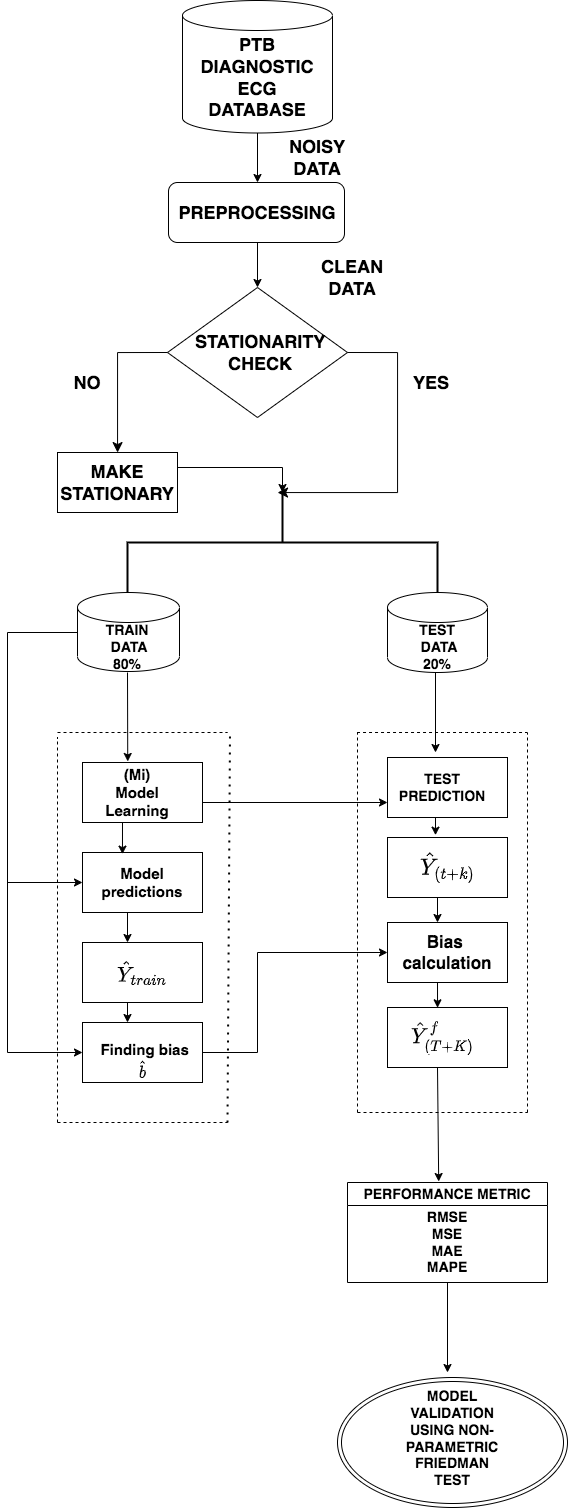
\includegraphics[scale=.3]{1.png}
          \caption{Flowchart of proposed2 (RB-GRU-CNN) model,  where GRU-CNN proposed model may utilize at model learning ($M_i$)}
  	\label{Fig:11}
  \end{figure*}

Workflow can be understood with the following flowchart as shown in Figure 6. The data is cleaned and all the null values are removed. An alpha=0.05 statistical test called the Friedman test is applied. Searches involving ECG,  DL and Artificial Intelligence are performed in conjunction to maximize sensitivity. The following criteria were used for inclusion with the following conditions: 1) Authentic DL studies involving ECG investigations. 2)A well-defined ECG dataset and a detailed description of DL techniques. There were exclusions if studies did not use DL with ECG dataset. The type of DL technique and results in form of error are extracted from each article.


The ability of DL models to predict ECG with minimum errors is studied. Individually applied base models like CNN, RNN, GRU, LSTM and BiLSTM. Single lead- 2  Datasets taken from Physionet website are cleaned and preprocessed. Stationarity of the dataset is checked to stationarize our datasets. Further our data is split into training and testing set. The 80\% data is used for training purpose and the rest 20\% for testing purpose. Although training and testing has been checked with various splittings just to try understand and make sure that no feature completely lies inside a single split. Same features have to be present in both training and testing sets just so our model catches the right references in order to predict. That being told is a major reason behind our model overfitting.
Further we fed this data individually to basic models and ran 20 iterations per data per model. Amongst these 20 iterations the predictions corresponding to the best The Root Mean Squared Error (RMSE) is stored. A final table corresponding to these performance metric is being made by taking mean of individually ran tables on multiple iterations. Researcher also performed a calculative test for deciding with how much percentile  proposed model is working better than basic models on all performance measures whose equations are given in (equation 17, equation 18, equation 19 and equation 20).


(RMSE),  Mean Squared Error(MSE),  Mean Absolute Error(MAE) and Mean Absolute Percent Error(MAPE) is defined as follows:

\begin{equation}
  {RMSE} = \sqrt{\frac{1}{m}\sum_{t=1}^{m}(x_t - \hat{y}_{t}^f)^2}
\end{equation}

\begin{equation}
  {MSE} = \frac{1}{m} \sum_{t=1}^{m} (x_t - \hat{y}_{t}^f)^2
\end{equation}
\begin{equation}
  {MAE} = \frac{1}{m} \sum_{t=1}^{m} \left|x_t - \hat{y}_{t}^f\right|
\end{equation}
\begin{equation}
  {MAPE} =\frac{100}{m} \sum_{t=1}^{m} \left| \frac{x_t - \hat{y}_{t}^f}{x_t} \right|
\end{equation}

where:
\begin{itemize}
  \item $m$ is the total number of data points, 
  \item $x_t$ is the true (observed) value for the $t$-th data point,  and
  \item $\hat{y}_{t}^f$ is the predicted value for the $t$-th data point.
\end{itemize}


Essentially, the RMSE is a commonly used statistic for calculating the average size of errors between predicted and actual values in a model. The square root of the average of the squared discrepancies between predicted and actual values is used to calculate it. RMSE weights greater errors more heavily,  making it susceptible to outliers. The average squared difference between predicted and actual values in a model is measured by MSE. The average of the squared discrepancies between predicted and actual values is used to calculate it. The average absolute difference between predicted and actual values in a model is measured by MAE. When compared to RMSE and MSE,  it is less sensitive to outliers because it handles all errors equally. MAPE is a metric for calculating a method's \% accuracy. It computes the average percentage difference between expected and actual values in relation to the predicted values. 








Several commonly used neural networks were used as contrast models to evaluate the performance and stability of the GRU-CNN model,  including the CNN,  GRU,  LSTM ,  BiLSTM ,  and RNN. In CNN,  GRU,  LSTM,  BiLSTM and RNN models,  the parameters were obtained from the training datasets and tested on the test dataset. A loss function provides a value for the degree of learning when used to evaluate if a prediction model is well trained and learned. Cross entropy,  which defines the separation among two probability distributions,  represents the loss function.
When the cross entropy is low,  the two probability distributions are more close. The formula for cross-entropy is shown below in (eq 21) :

\begin{equation}
  {Loss} =- \frac{1}{m} \sum_{t=1}^{m} \left( x_t \log(\hat{y}_{t}^f) + (1 - x_t) \log(1 - \hat{y}_{t}^f) \right)
\end{equation}

where $m$ is the number of data points,  $x_t$ is the true label (ground truth) of the $t$-th data point,  and $\hat{y}_{t}^f$ is the predicted probability (output) of the $t$-th data point belonging to the positive class.
Training sets fit better when loss values are closer to zero.
It can be see from loss plot Figure 7 that loss values for the chosen models are very close to zero. \\ Now that model is trained,  testing is being performed on unseen 20\% data. Then prediction errors are calculated based on testing performance.

  \begin{figure*}[h!]
   \centering
   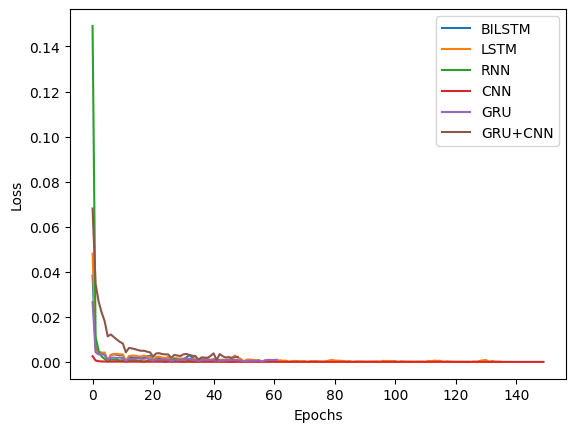
\includegraphics[scale=.5]{val_loss.png}
    \caption{Training losses of BiLSTM, LSTM, RNN, CNN, GRU \& Proposed GRU-CNN models corresponding to the epochs}
    \label{Fig:12}
  \end{figure*}



Proposed-1 has been shown to perform better than the other basic DL models in terms of RMSE, MSE, MAE \& MAPE.  Also discovered is \%imp, which indicates what percentage of the proposed model (Proposed 1) outperforms the implemented classical DL models.


The percentage improvement in RMSE is calculated as:
\begin{equation}
    \text{RMSE}_{\%imp} = \frac{\text{M(i)}_{\text{RMSE}} - \text{Proposed}_{\text{RMSE}}}{\text{M(i)}_{\text{RMSE}}/100}
\end{equation}

where $\text{M(i)}_{\text{RMSE}}$ is the basic model's RMSE,  and $\text{Proposed}_{\text{RMSE}}$ is the RMSE of proposed Model. `\\`

The percentage improvement in MSE is calculated as:
\begin{equation}
    \text{MSE}_{\%imp} = \frac{\text{M(i)}_{\text{MSE}} - \text{Proposed}_{\text{MSE}}}{\text{M(i)}_{\text{MSE}}/100}
\end{equation}

where $\text{M(i)}_{\text{MSE}}$ is the basic model's MSE,  and $\text{Proposed}_{\text{MSE}}$ is the MSE of proposed model. `\\`

The percentage improvement in MAE is calculated as:
\begin{equation}
    \text{MAE}_{\%imp} = \frac{\text{M(i)}_{\text{MAE}} - \text{Proposed}_{\text{MAE}}}{\text{M(i)}_{\text{MAE}}/100}
\end{equation}

where $\text{M(i)}_{\text{MAE}}$ is the basic model's MAE,  and $\text{Proposed}_{\text{MAE}}$ is the MAE of proposed model. `\\`

The percentage improvement in MAPE is calculated as:
\begin{equation}
   \text{MAPE}_{\%imp} = \frac{\text{M(i)}_{\text{MAPE}} - \text{Proposed}_{\text{MAPE}}}{\text{M(i)}_{\text{MAPE}}/100}
\end{equation}

where $\text{M(i)}_{\text{MAPE}}$ is the basic model's MAPE,  and $\text{Proposed}_{\text{MAPE}}$ is the MAPE of proposed model.







% 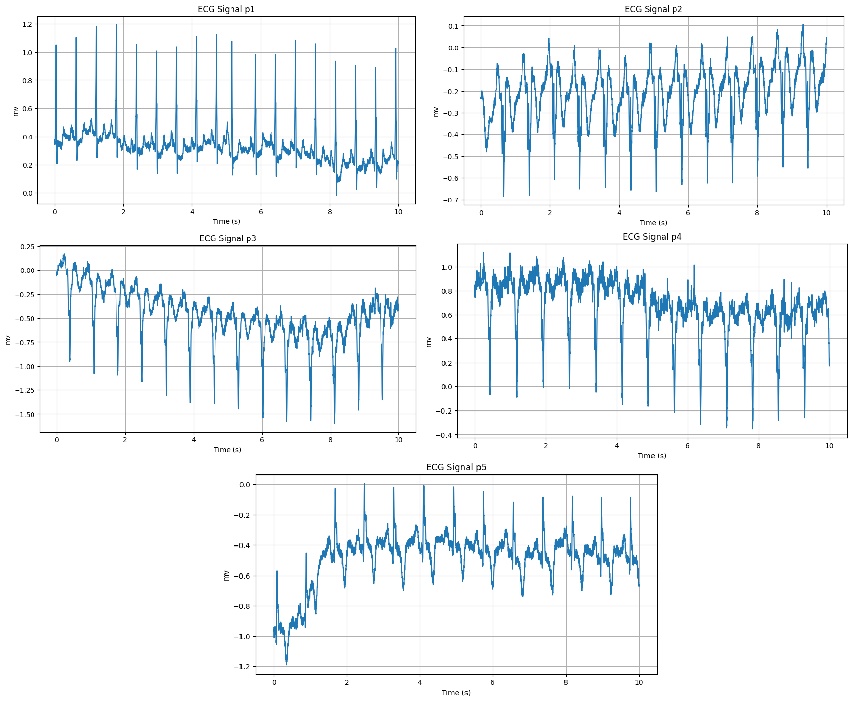
\includegraphics[scale=.7]{edadrawio.pdf}

% \begin{landscape}

%\end{landscape}







\begin{comment}
\begin{table*}[htbp]
  \centering
  \caption{The performance RMSE of standalone DL Models and proposed GRU-CNN}
  \label{tab:Table 1}
  \begin{tabular}{|c|c|c|c|c|c|c|c|c|c|c|c|}
    \hline
    & CNN & RNN &  LSTM & GRU & BiLSTM  & Pro 1 & Pro 2\\
    \hline
    D1 & 0.02511 & 0.029045 & 0.02845 & 0.023255 & 0.026725 & 0.017375 & 0.017246\\
    D2 & 0.048335 & 0.05851 & 0.033775 & 0.044645 & 0.054565 & 0.016211 & 0.01425\\
    D3 & 0.07086 & 0.07155 & 0.07388 & 0.069305 & 0.08139 & 0.04781 & 0.04211 \\
    D4 & 0.053515 & 0.05766 & 0.054275 & 0.051595 & 0.05713 & 0.048195 & 0.040361\\
    D5 & 0.04291 & 0.02836 & 0.02967 & 0.07155 & 0.07086 & 0.02017 & 0.02\\
    Mean & 0.048146 & 0.049025 & 0.04401 & 0.05207 & 0.058134 & 0.0299522 & 0.0267934 \\
    \hline
  \end{tabular}
\end{table*}
In table \ref{tab:Table 1},  we can see that an average RMSE of 0.04816,  0.049025,  0.04401,  0.05207,  0.058134 and 0.0299522 is achived by CNN,  RNN,  LSTM,  GRU,  BiLSTM and Pro1. We have also seen in table \ref{tab:Table 2} percentage improvement of 38.54\%,  38.18\%,  33.88\%,  37.33\% and 46.74\% in Pro1 with respect to CNN,  RNN,  LSTM,  GRU and BiLSTM. LSTM is the second best performing model after Pro1 while BiLSTM is giving maximum RMSE taking the last position among rest.
\begin{table*}[htbp]
  \centering
  \caption{Percentage improvement of standalone DL Models corresponding to proposed GRU-CNN}
  \label{tab:Table 2}
  \begin{tabular}{|c|c|c|c|c|c|c|c|c|c|c|c|}
    \hline
    & \% imp CNN & \% imp RNN & \% imp LSTM & \% imp GRU & \% imp BiLSTM \\
    \hline
    D1 & 30.80\% & 40.17\% & 38.92\% & 25.28\% & 34.98\% \\
    D2 & 66.46\% & 72.29\% & 52\% & 52\% & 70.29\%\\
    D3 & 32.52\% & 33.17\% & 35.28\% & 31.01\% & 41.25\%\\
    D4 & 9.94\% & 16.41\% & 11.20\% & 6.58\% & 15.63\%\\
    D5 & 52.99\% & 28.87\% & 32\% & 71.80\% & 71.53\%\\
    Mean & 38.54\% & 38.18\% & 33.88\% & 37.33\% & 46.74\%\\
    \hline
  \end{tabular}
\end{table*}
\begin{table*}[htbp]
  \centering
  \caption{The performance MSE of standalone DL Models and proposed GRU-CNN}
  \label{tab:Table 3}
  \begin{tabular}{|c|c|c|c|c|c|c|c|c|c|c|c|}
    \hline
    & CNN & RNN & LSTM &  GRU &  BiLSTM & Pro 1 & Pro 2\\
    \hline
    D1 & 0.000625 & 0.000905 & 0.00085 & 0.000555 & 0.00074 & 0.000315 & 0.000286\\
    D2 & 0.00236 & 0.003575 & 0.00118 & 0.002035 & 0.006135 & 0.000315 & 0.00029\\
    D3 & 0.00505 & 0.00577 & 0.005465 & 0.00483 & 0.00662 & 0.002345 & 0.00219 \\
    D4 & 0.002925 & 0.00359 & 0.002965 & 0.002685 & 0.00328 & 0.002335 & 0.00202\\
    D5 & 0.00204 & 0.00082 & 0.00089 & 0.00577 & 0.00505 & 0.00042 & 0.00031 \\
    Mean & 0.0026 & 0.002932 & 0.00227 & 0.003175 & 0.004365 & 0.001146 & 0.0010192\\
    \hline
  \end{tabular}
\end{table*}
In table \ref{tab:Table 3},  we can see that an average MSE of 0.0026,  0.002932,  0.00227,  0.003175,  0.004365 and 0.001146 is achived by CNN,  RNN,  LSTM,  GRU,  BiLSTM and Pro1. We have also seen in table \ref{tab:Table 4} percentage improvement of 57.88\%,  59.89\%,  53.47\%,  56.99\% and 67.46\% in Pro1 with respect to CNN,  RNN,  LSTM,  GRU and BiLSTM. LSTM is the second best performing model after Pro1 while BiLSTM is giving maximum MSE taking the last position among rest.
\begin{table*}[htbp]
  \centering
  \caption{Percentage improvement of standalone DL Models corresponding to proposed GRU-CNN}
  \label{tab:Table 4}
  \begin{tabular}{|c|c|c|c|c|c|c|c|c|c|c|c|}
    \hline
    & \% imp CNN & \% imp RNN & \% imp LSTM & \% imp GRU & \% imp BiLSTM \\
    \hline
    D1 & 49.60\% & 65.19\% & 62.94\% & 43.24\% & 57.43\% \\
    D2 & 86.65\% & 91.18\% & 73.30\% & 84.52\% & 94.86\%\\
    D3 & 53.56\% & 59.35\% & 57.09\% & 51.44\% & 64.57\%\\
    D4 & 20.17\% & 34.95\% & 21.24\% & 13.03\% & 28.81\%\\
    D5 & 79.41\% & 48.78\% & 52.80\% & 92.72\% & 91.63\%\\
    Mean & 57.88\% & 59.89\% & 53.47\% & 56.99\% & 67.46\%\\
    \hline
  \end{tabular}
\end{table*}


\begin{table*}[htbp]
  \centering
  \caption{The performance MAE of standalone DL Models and proposed GRU-CNN}
  \label{tab:Table 5}
  \begin{tabular}{|c|c|c|c|c|c|c|c|c|c|c|c|}
    \hline
    & CNN & RNN & LSTM &  GRU &  BiLSTM & Pro 1 & Pro 2\\
    \hline
    D1 & 0.011715 & 0.01838 & 0.01557 & 0.012045 & 0.01579 & 0.00956 & 0.00852\\
    D2 & 0.03676 & 0.04618 & 0.01851 & 0.03445 & 0.0415 & 0.00811 & 0.0072\\
    D3 & 0.04694 & 0.044345 & 0.048095 & 0.043585 & 0.0491 & 0.03033 & 0.02318\\
    D4 & 0.035295 & 0.03525 & 0.03449 & 0.032885 & 0.034545 & 0.03131 & 0.02336\\
    D5 & 0.02873 & 0.018095 & 0.018915 & 0.044345 & 0.04694 & 0.011685 & 0.0045\\
    Mean & 0.031888 & 0.03245 & 0.027116 & 0.033462 & 0.037575 & 0.018199 & 0.013352 \\
    \hline
  \end{tabular}
\end{table*}
In table \ref{tab:Table 5},  we can see that an average MAE of 0.031888,  0.03245,  0.027116,  0.033462,  0.037575 and 0.018199 is achived by CNN,  RNN,  LSTM,  GRU,  BiLSTM and Pro1. We have also seen in table \ref{tab:Table 6} percentage improvement of 40.46\%,  41.72\%,  35.83\%,  41.18\% and 48.52\% in Pro1 with respect to CNN,  RNN,  LSTM,  GRU and BiLSTM. LSTM is the second best performing model after Pro1 while BiLSTM is giving maximum MAE taking the last position among rest.
\begin{table*}[htbp]
  \centering
  \caption{Percentage improvement of standalone DL Models corresponding to proposed GRU-CNN}
  \label{tab:Table 6}
  \begin{tabular}{|c|c|c|c|c|c|c|c|c|c|c|c|}
    \hline
    & \% imp CNN & \% imp RNN & \% imp LSTM & \% imp GRU & \% imp BiLSTM \\
    \hline
    D1 & 18.39\% & 47.98\% & 38.59\% & 20.63\% & 39.45\% \\
    D2 & 77.93\% & 82.43\% & 56.18\% & 76.45\% & 80.45\%\\
    D3 & 35.38\% & 31.60\% & 36.93\% & 30.41\% & 38.22\%\\
    D4 & 11.29\% & 11.17\% & 9.22\% & 4.78\% & 9.36\%\\
    D5 & 59.32\% & 35.42\% & 38.22\% & 73.64\% & 75.10\%\\
    Mean & 40.46\% & 41.72\% & 35.83\% & 41.18\% & 48.52\%\\
    \hline
  \end{tabular}
\end{table*}

\begin{table*}[htbp]
  \centering
  \caption{The performance MAPE of standalone DL Models and proposed GRU-CNN}
  \label{tab:Table 7}
  \begin{tabular}{|c|c|c|c|c|c|c|c|c|c|c|c|}
    \hline
    & CNN & RNN & LSTM &  GRU &  BiLSTM & Pro 1 & Pro 2\\
    \hline
    D1 & 5.758535 & 9.3428 & 7.472155 & 5.433125 & 7.69268 & 4.65592 & 3.22098\\
    D2 & 6.144505 & 7.40371 & 9.10457 & 5.852235 & 6.849115 & 3.82211 & 3.2145 \\
    D3 & 9.79425 & 10.242305 & 9.93871 & 9.85453 & 10.8904 & 5.962575 & 4.376\\
    D4 & 8.24417 & 9.73791 & 8.29686 & 8.59091 & 9.001425 & 6.950645 & 4.2018\\
    D5 & 4.98369 & 8.88995 & 5.698585 & 10.242305 & 9.79425 & 3.14022 & 3.11067\\
    Mean & 6.98503 & 9.123335 & 8.102176 & 7.994621 & 8.845574 & 4.906294 & 3.62479\\
    \hline
  \end{tabular}
\end{table*}
In table \ref{tab:Table 7},  we can see that an average MAPE of 6.98503,  9.123335,  8.102176,  7.994621,  8.845574 and 4.906294 is achived by CNN,  RNN,  LSTM,  GRU,  BiLSTM and Pro1. We have also seen in table \ref{tab:Table 8} percentage improvement of 29.75\%,  46.72\%,  39.36\%,  35.38\% and 43.92\% in Pro1 with respect to CNN,  RNN,  LSTM,  GRU and BiLSTM. CNN is the second best performing model after Pro1 while RNN is giving maximum MAPE taking the last position among rest.
\begin{table*}[htbp]
  \centering
  \caption{Percentage improvement of standalone DL Models corresponding to proposed GRU-CNN}
  \label{tab:Table 8}
  \begin{tabular}{|c|c|c|c|c|c|c|c|c|c|c|c|}
    \hline
    & \% imp CNN & \% imp RNN & \% imp LSTM & \% imp GRU & \% imp BiLSTM \\
    \hline
    D1 & 19.14\% & 50.16\% & 37.68\% & 14.30\% & 39.47\% \\
    D2 & 37.79\% & 48.37\% & 58.01\% & 34.68\% & 44.19\%\\
    D3 & 39.12\% & 41.78\% & 40\% & 39.49\% & 45.24\%\\
    D4 & 15.69\% & 28.62\% & 16.22\% & 19.09\% & 22.78\%\\
    D5 & 36.99\% & 64.67\% & 44.89\% & 69.34\% & 67.93\%\\
    Mean & 29.75\% & 46.72\% & 39.36\% & 35.38\% & 43.92\%\\
    \hline
  \end{tabular}
\end{table*}
\end{comment}






\section{Results and Analysis}

\subsection{Quantitative Analysis}



\begin{table}[!p]
    \centering
    \caption{Performances of traditional DL models and both proposed models(i.e,  GRU-CNN(proposed-1)) and RB-GRU-CNN(proposed-2)) based on RMSE,  MSE,  MAE and MAPE measures over PTB diagnostic ECG datasets.}
    \label{tab:error_metrics}
    \begin{tabular}{ccccccccc}
        \toprule
        Error Metric & Dataset & CNN & RNN & LSTM & GRU & BiLSTM & PRO-1 & PRO-2 \\
        \midrule
        \multirow{9}{*}{RMSE} \\
        & D1 & 0.02511 & 0.029045 & 0.02845 & 0.023255 & 0.026725 & 0.017375 & 0.017246 \\
        & D2 & 0.048335 & 0.05851 & 0.033775 & 0.044645 & 0.054565 & 0.016211 & 0.01425 \\
        & D3 & 0.07086 & 0.07155 & 0.07388 & 0.069305 & 0.08139 & 0.04781 & 0.04211\\
        & D4 & 0.053515 & 0.05766 & 0.054275 & 0.051595 & 0.05713 & 0.048195 & 0.040361\\
        & D5 & 0.04291 & 0.02836 & 0.02967 & 0.07155 & 0.07086 & 0.02017 & 0.02\\
        & Mean & 0.048146 & 0.049025 & 0.04401 & 0.05207 & 0.058134 & 0.0299522 & 0.0267934 \\
        \midrule
        \multirow{9}{*}{MSE}\\
        & D1 & 0.000625 & 0.000905 & 0.00085 & 0.000555 & 0.00074 & 0.000315 & 0.000286 \\
        & D2 & 0.00236 & 0.003575 & 0.00118 & 0.002035 & 0.006135 & 0.000315 & 0.00029\\
        & D3 & 0.00505  & 0.00577 & 0.005465 & 0.00483 & 0.00662 & 0.002345 & 0.00219 \\
        & D4 & 0.002925 & 0.00359 & 0.002965 & 0.002685 & 0.00328 & 0.002335 & 0.00202 \\
        & D5 & 0.00204 & 0.00082 & 0.00089 & 0.00577 & 0.00505 & 0.00042 & 0.00031 \\
        & Mean & 0.0026 & 0.002932 & 0.00227 & 0.003175 & 0.004365 & 0.001146 & 0.0010192 \\
        \midrule
        \multirow{9}{*}{MAE}\\
        & D1 & 0.011715 & 0.01838 & 0.01557 & 0.012045 & 0.01579 & 0.00956 & 0.00852 \\
        & D2 & 0.03676 & 0.04618 & 0.01851 & 0.03445 & 0.0415 & 0.00811 & 0.0072 \\
        & D3 & 0.04694 & 0.044345 & 0.048095 & 0.043585 & 0.0491 & 0.03033 & 0.02318 \\
        & D4 & 0.035295 & 0.03525 & 0.03449 & 0.032885 & 0.034545 & 0.03131 & 0.02336 \\
        & D5  & 0.02873 & 0.018095 & 0.018915 & 0.044345 & 0.04694 & 0.011685 & 0.0045 \\
        & Mean & 0.031888 & 0.03245 & 0.027116 & 0.033462 & 0.037575 & 0.018199 & 0.013352 \\
        \midrule
        \multirow{9}{*}{MAPE}\\
        & D1 & 5.758535 & 9.3428 & 7.472155 & 5.433125 & 7.69268 & 4.65592 & 3.22098 \\
        & D2 & 6.144505 & 7.40371 & 9.10457 & 5.852235 & 6.849115 & 3.82211 & 3.2145 \\
        & D3 & 9.79425 & 10.242305 & 9.93871 & 9.85453 & 10.8904 & 5.962575 & 4.376 \\
        & D4 & 8.24417 & 9.73791 & 8.29686 & 8.59091 & 9.001425 & 6.950645 & 4.2018 \\
        & D5 & 4.98369 & 8.88995 & 5.698585 & 10.242305 & 9.79425 & 3.14022 & 3.11067 \\
        & Mean & 6.98503 & 9.123335 & 8.102176 & 7.994621 & 8.845574 & 4.906294 & 3.62479 \\
       
        \bottomrule
    \end{tabular}
\end{table}

\begin{table}[!h]
    \centering
    \caption{Percentage improvement over traditional models based on proposed-1 GRU-CNN model for RMSE,  MSE,  MAE and MAPE measures.}
    \label{tab:error_metrics}
    \begin{tabular}{ccccccc}
        \toprule
        Error Metric & Dataset & \%imp CNN & \%imp RNN & \%imp LSTM & 
        \%imp GRU & \%imp BiLSTM \\
        \midrule
        \multirow{7}{*}{RMSE} \\
        & D1 & 30.80\% & 40.17\% & 38.92\% & 25.28\% & 34.98\% \\
        & D2 & 66.46\% & 72.29\% & 52\% & 52\% & 70.29\% \\
        & D3 & 32.52\% & 33.17\% & 35.28\% & 31.01\% & 41.25\% \\
        & D4 & 9.94\% & 16.41\% & 11.20\% & 6.58\% & 15.63\%\\
        & D5 & 52.99\% & 28.87\% & 32\% & 71.80\% & 71.53\%\\
        & Mean & 38.54\% & 38.18\% & 33.88\% & 37.33\% & 46.74\%\\
        \midrule
        \multirow{7}{*}{MSE}\\
        & D1 & 49.60\% & 65.19\% & 62.94\% & 43.24\% & 57.43\%\\
        & D2 & 86.65\% & 91.18\% & 73.30\% & 84.52\% & 94.86\%\\
        & D3 & 53.56\%  & 59.35\% & 57.09\% & 51.44\% & 64.57\%\\
        & D4 & 20.17\% & 34.95\% & 21.24\% & 13.03\% & 28.81\%\\
        & D5 & 79.41\% & 48.78\% & 52.80\% & 92.72\% & 91.63\%\\
        & Mean & 57.88\% & 59.89\% & 53.47\% & 56.99\% & 67.46\%\\
        \midrule
        \multirow{7}{*}{MAE}\\
        & D1 & 18.39\% & 47.98\% & 38.59\% & 20.63\% & 39.45\%\\
        & D2 & 77.93\% & 82.43\% & 56.18\% & 76.45\% & 80.45\%\\
        & D3 & 35.38\% & 31.60\% & 36.93\% & 30.41\% & 38.22\%\\
        & D4 & 11.29\% & 11.17\% & 9.22\% & 4.78\% & 9.36\%\\
        & D5  & 59.32\% & 35.42\% & 38.22\% & 73.64\% & 75.10\%\\
        & Mean & 40.46\% & 41.72\% & 35.83\% & 41.18\% & 48.52\%\\
        \midrule
        \multirow{7}{*}{MAPE}\\
        & D1 & 19.14\% & 50.16\% & 37.68\% & 14.30\% & 39.47\%\\
        & D2 & 37.79\% & 48.37\% & 58.01\% & 34.68\% & 44.19\%\\
        & D3 & 39.12\% & 41.78\% & 40\% & 39.49\% & 45.24\%\\
        & D4 & 15.69\% & 28.62\% & 16.22\% & 19.09\% & 22.78\%\\
        & D5 & 36.99\% & 64.67\% & 44.89\% & 69.34\% & 67.93\%\\
        & Mean & 29.75\% & 46.72\% & 39.36\% & 35.38\% & 43.92\%\\ 
        \bottomrule
    \end{tabular}
\end{table}  

It can be seen in Table 1 that on taking four performance metrics the 5 datasets when fed to traditional DL models and compared with proposed-1,  turns out proposed-1 is outperforming implemented traditional models. Proposed-1 is giving least RMSE compared to traditional DL models. Proposed-1(GRU-CNN) on all 5 datasets gave a mean value of RMSE 0.0299522 . A major \% improvement in proposed-1 with respect to traditional DL models can be seen in Table 2 where models CNN,  RNN,  LSTM,  GRU and BiLSTM shown a percentage improvement of 38.54\%,  38.18\%,  33.88\%,  37.33\% and 46.74\% respectively,  which are mean values of \% improvement in RMSE corresponding to datasets with respect to proposed-1 model. Quantitatively proposed-2 is giving less RMSE than proposed-1,  for the model proposed-2 on all 5 datasets a mean value of RMSE 0.0267934 is achieved hence,  it can be concluded that proposed-2 is better than proposed-1 since RMSE of proposed-2 is less than RMSE of proposed-1. 

Similarly,  from Table 1, it can be observed that  Proposed-1 is giving least MSE compared to traditional DL models. Proposed-1 on all 5 datasets gave a mean value of MSE 0.001146 . A major \% improvement in proposed-1 with respect to traditional DL models can be seen in Table 2 where models CNN,  RNN,  LSTM,  GRU and BiLSTM shown a percentage improvement of 57.88\%,  59.89\%,  53.47\%,  56.99\% and 67.46\% respectively,  which are mean values of \% improvement in MSE corresponding to datasets with respect to proposed-1 model. Quantitatively proposed-2 is giving less MSE than proposed-1,  for the model proposed-2 on all 5 datasets a mean value of MSE 0.0010192 is achieved hence,  it can be concluded that proposed-2 is better than proposed-1 since,  MSE of proposed-2 is less than MSE of proposed-1. 

Again,  from Table 1 it can be observed that  Proposed-1 is giving least MAE compared to traditional DL models. Proposed-1 on all 5 datasets gave a mean value of MAE 0.018199 . A major \% improvement in proposed-1 with respect to traditional DL models can be seen in Table 2 where models CNN,  RNN,  LSTM,  GRU and BiLSTM shown a percentage improvement of 40.46\%,  41.72\%,  35.83\%,  41.18\% and 48.52\% respectively,  which are mean values of \% improvement in MAE corresponding to datasets with respect to proposed-1 model. Quantitatively proposed-2 is giving less MAE than proposed-1,  for the model proposed-2 on all 5 datasets a mean value of MAE 0.013352 is achieved Hence,  it can be concluded that proposed-2 is better than proposed-1 since MAE of proposed-2 is less than MAE of proposed-1.

At last,  from Table 1 it can be observed that  Proposed-1 is giving least MAPE compared to traditional DL models. Proposed-1 on all 5 datasets gave a mean value of MAPE 4.906294 . A major \% improvement in proposed-1 with respect to traditional DL models can be seen in Table 2 where models CNN,  RNN,  LSTM,  GRU and BiLSTM shown a percentage improvement of 29.75\%,  46.72\%,  39.36\%,  35.38\% and 43.92\% respectively,  which are mean values of \% improvement in MAPE corresponding to datasets with respect to proposed-1 model. Quantitatively proposed-2 is giving less MAPE than proposed-1,  for the model proposed-2 on all 5 datasets a mean value of MAPE 3.62479 is achieved hence,  it can be concluded that proposed-2 is better than proposed-1 since MAPE of proposed-2 is less than MAPE of proposed-1.
 \begin{figure*}[h!]
   \centering
   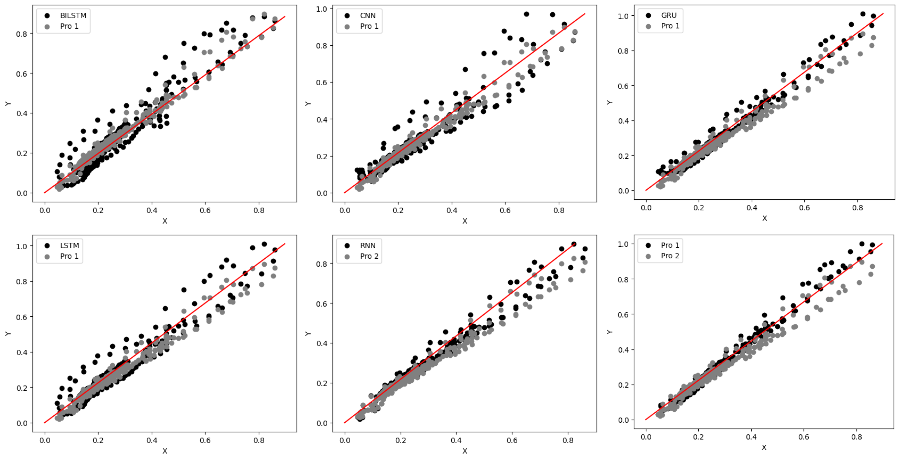
\includegraphics[scale=.5]{d1_sp.drawio.png}
     %\captionsetup{justification=centering, margin=2cm}
    \caption{Scatter plots of proposed GRU-CNN(pro-1) with stand alone DL models along with proposed-2 RB-GRU-CNN(pro-2), where x-axis \& y-axis represent the predictions of models and original test data D1.}
    \label{Fig:6}
   \end{figure*}
   \begin{figure*}[h!]
    \centering
     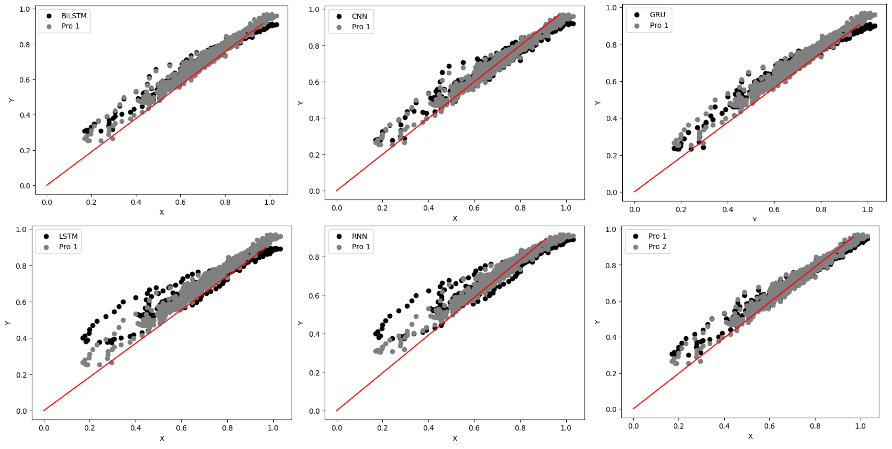
\includegraphics[scale=.5]{d2_sp.drawio.png}
     \caption{Scatter plots of proposed GRU-CNN(pro-1) with stand alone DL models along with proposed-2 RB-GRU-CNN(pro-2), where x-axis \& y-axis represent the predictions of models and original test data D2.}
     \label{Fig:7}
  \end{figure*}
  \begin{figure*}[h!]
     \centering
     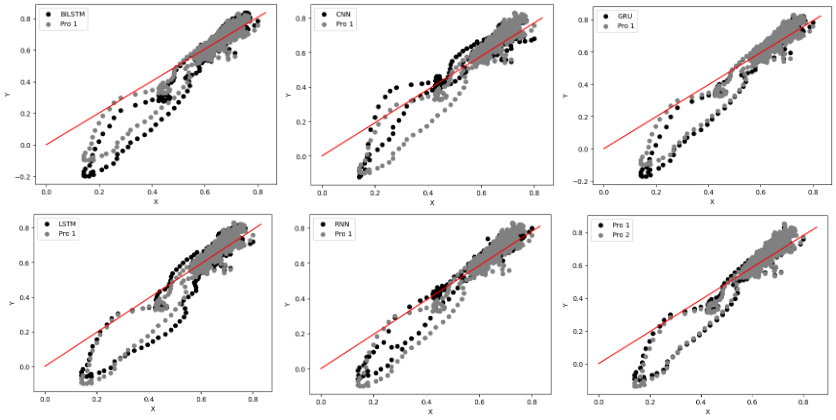
\includegraphics[scale=.5]{d3_sp.drawio.png}
     \caption{Scatter plots of proposed GRU-CNN(pro-1) with stand alone DL models along with proposed-2 RB-GRU-CNN(pro-2), where x-axis \& y-axis represent the predictions of models and original test data D3.}
     \label{Fig:8}
   \end{figure*}
   \begin{figure*}[h!]
    \centering
     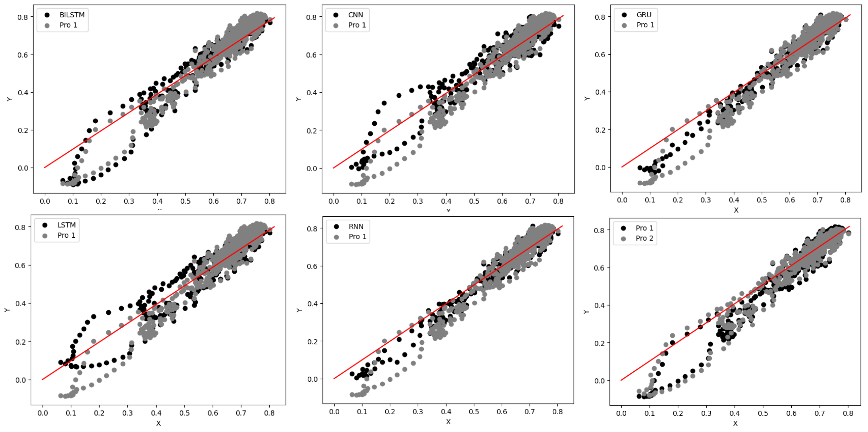
\includegraphics[scale=.5]{d4_sp.drawio.png}
     \caption{Scatter plots of proposed GRU-CNN(pro-1) with stand alone DL models along with proposed-2 RB-GRU-CNN(pro-2), where x-axis \& y-axis represent the predictions of models and original test data D4.}
     \label{Fig:9}
   \end{figure*}
   \begin{figure}[h!]
    \centering
     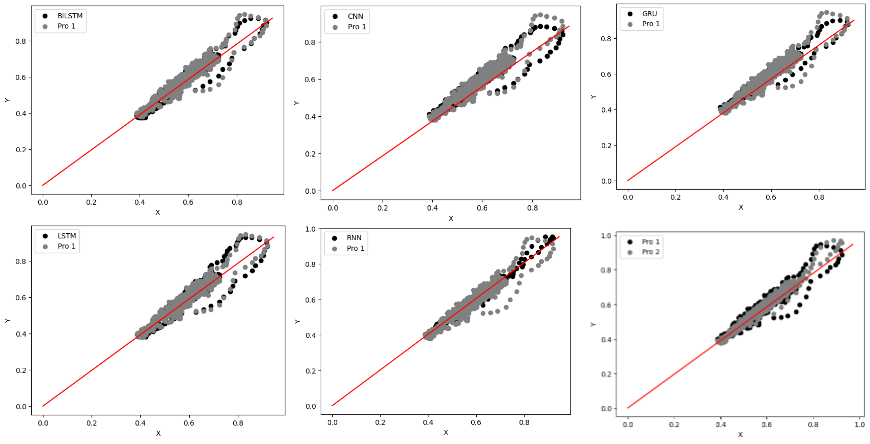
\includegraphics[scale=.5]{d5_sp.drawio.png}
     \caption{Scatter plots of proposed GRU-CNN(pro-1) with stand alone DL models along with proposed-2 RB-GRU-CNN(pro-2), where x-axis \& y-axis represent the predictions of models and original test data D5.}
     \label{Fig:10}
   \end{figure}

   \begin{figure*}[h!]
    \centering
     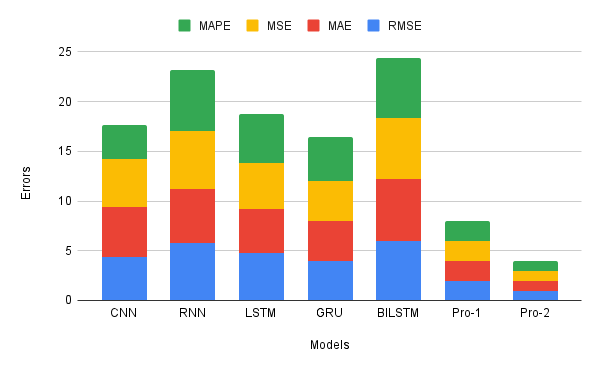
\includegraphics[scale=.6]{aggregator.png}
     \caption{Aggregate measures comparison of traditional models and proposed (pro-1 \& pro-2) models.}
     \label{Fig:13}
   \end{figure*} 
\subsection{Graphical Analysis}
 \begin{figure*}[h!]
    \centering
    \subfigure{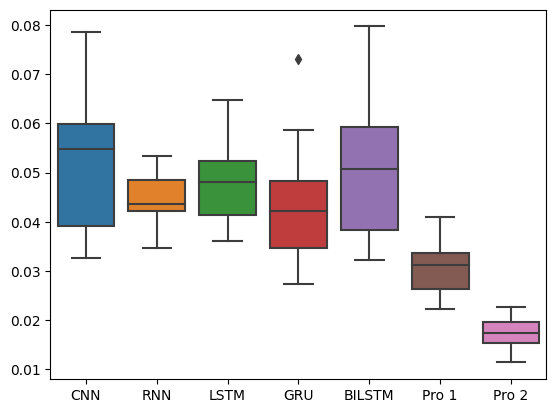
\includegraphics[scale=0.5]{d1rmse}}
    \subfigure{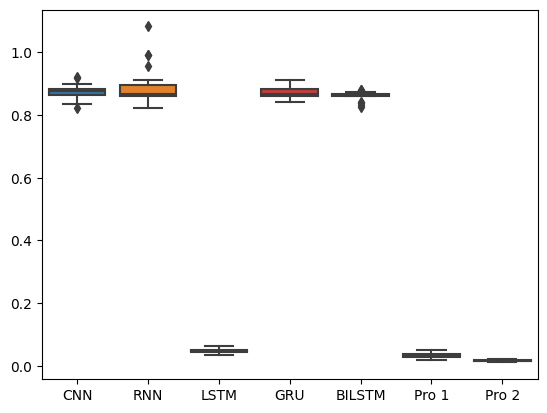
\includegraphics[scale=0.5]{D2_RMSE}}
    \subfigure{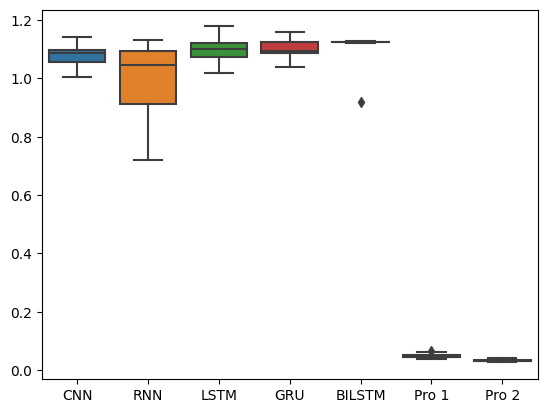
\includegraphics[scale=0.5]{D3_RMSE}}
    \subfigure{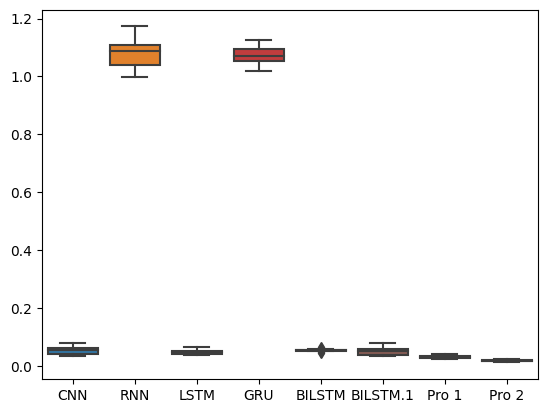
\includegraphics[scale=0.5]{d4_rmse}}
    \subfigure{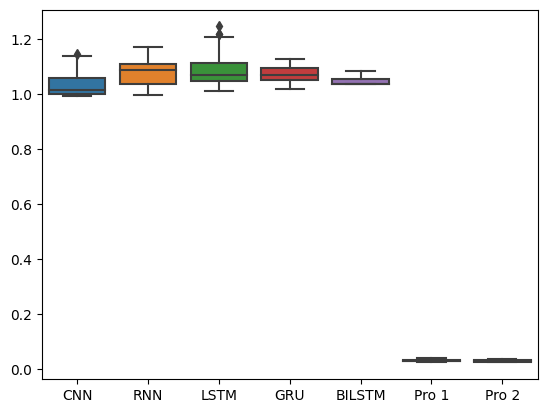
\includegraphics[scale=0.5]{D5_RMSE}}
    \caption{RMSE (performance box-plots) of basic DL models with proposed hybrid models (pro-1 \& pro-2).}
    \label{Fig:14}
  \end{figure*}

  \begin{figure*}[h!]
    \centering
    \subfigure{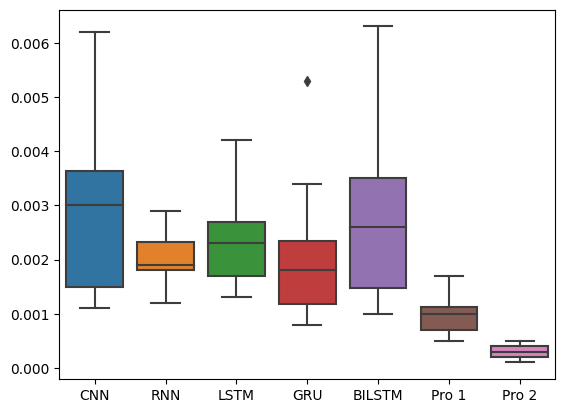
\includegraphics[scale=0.5]{d1_mse}}
    \subfigure{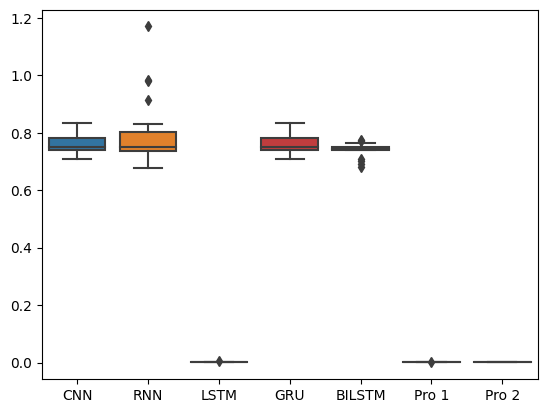
\includegraphics[scale=0.5]{D2_MSE}}
    \subfigure{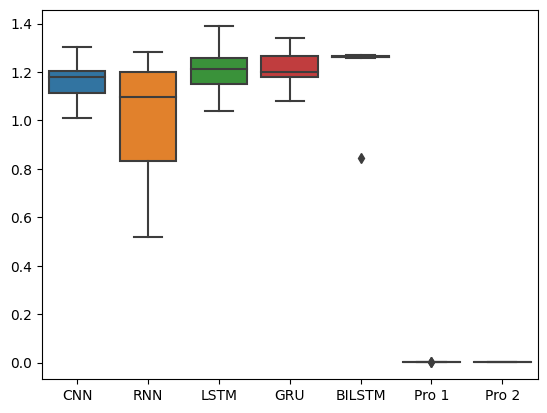
\includegraphics[scale=0.5]{D3_MSE}}
    \subfigure{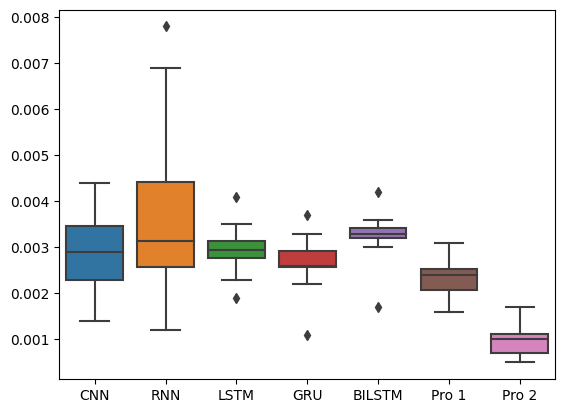
\includegraphics[scale=0.5]{d4_mse}}
    \subfigure{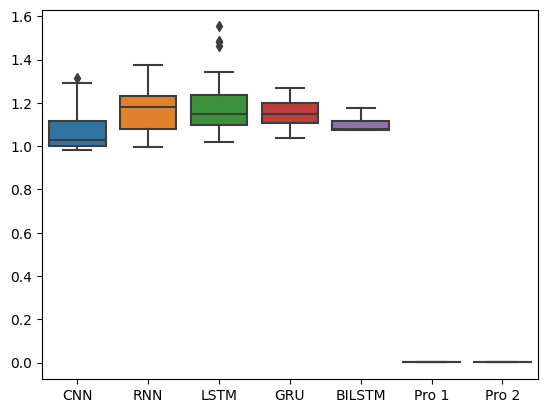
\includegraphics[scale=0.5]{D5_MSE}}
    \caption{MSE (performance box-plots) of basic DL models with proposed hybrid models (pro-1 \& pro-2).}
    \label{Fig:15}
  \end{figure*}

  \begin{figure*}[h!]
   \centering
    \subfigure{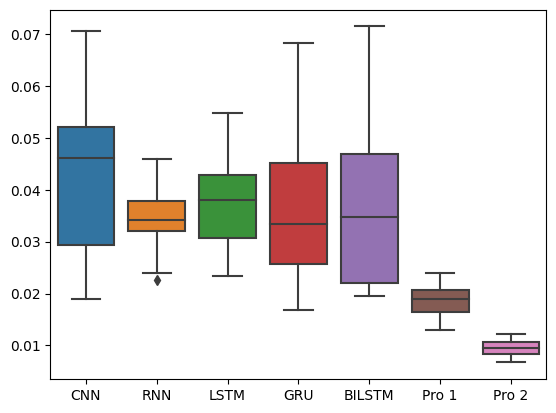
\includegraphics[scale=0.5]{d1_mae}} 
    \subfigure{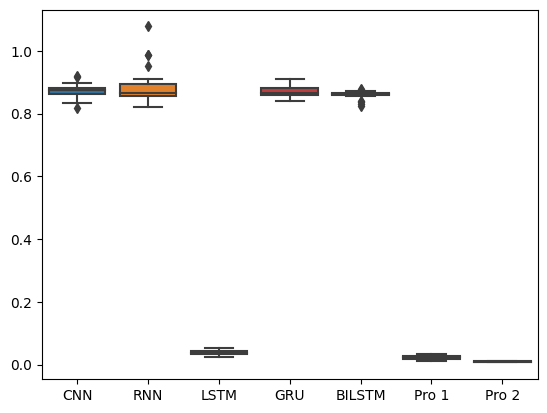
\includegraphics[scale=0.5]{D2_MAE}}
    \subfigure{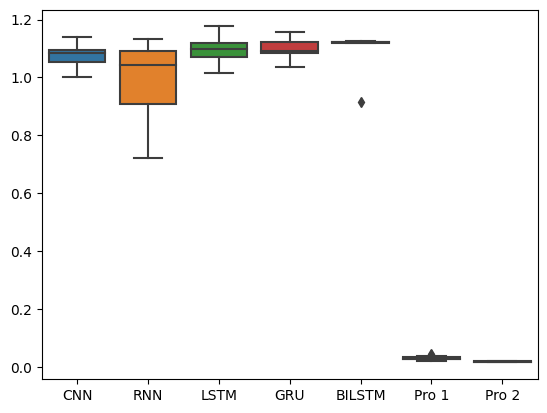
\includegraphics[scale=0.5]{D3_MAE}}
    \subfigure{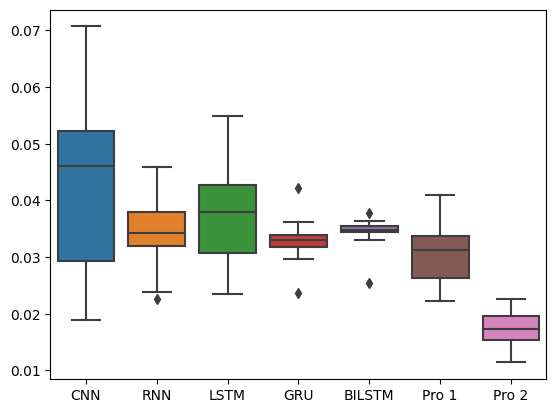
\includegraphics[scale=0.5]{d4_mae}}
    \subfigure{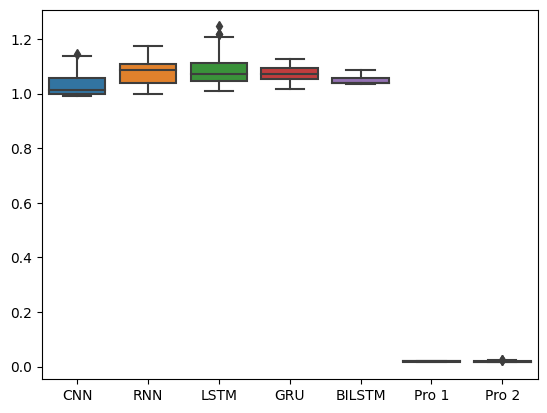
\includegraphics[scale=0.5]{D5_MAE}}
    \caption{MAE (performance box-plots) of basic DL models with proposed hybrid models (pro-1 \& pro-2).}
    \label{Fig:16}
  \end{figure*}
  \begin{figure*}[h!]
    \centering
    \subfigure{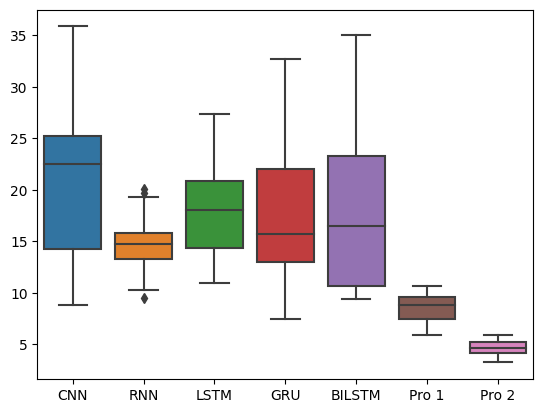
\includegraphics[scale=0.5]{d1_mape}}
    \subfigure{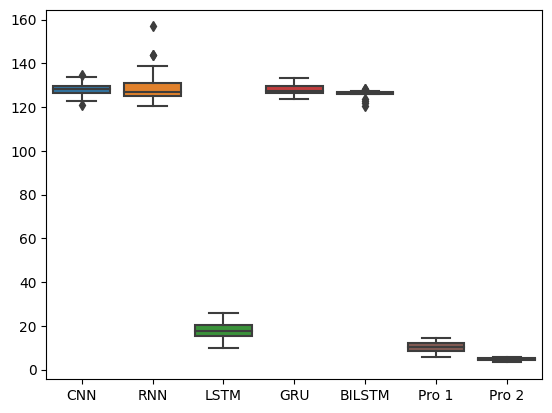
\includegraphics[scale=0.5]{D2_MAPE}}
    \subfigure{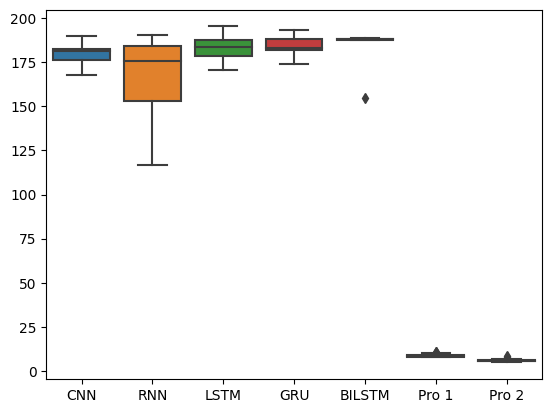
\includegraphics[scale=0.5]{D3_MAPE}}
    \subfigure{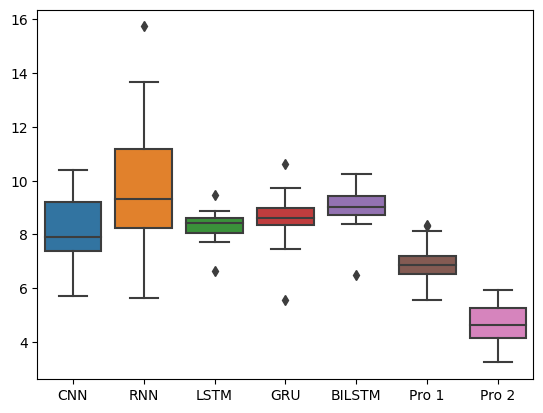
\includegraphics[scale=0.5]{d4_mape}} 
    \subfigure{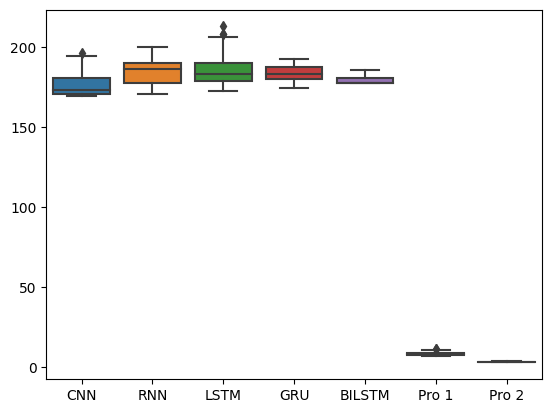
\includegraphics[scale=0.5]{D5_MAPE}}
    \caption{MAPE (performance box-plots) of basic DL models with proposed hybrid models (pro-1 \& pro-2).}
    \label{Fig:17}
  \end{figure*}
In this section graphical analysis of our experiments is shown. Overlaying the scatterplot is a line of regression with a distinct 45-degree angle. The angle indicates that there is a high positive correlation between the two variables,  implying a linear relationship. Two more regression lines are visible on the scatterplot upon closer scrutiny. One of these lines closely follows the general trend of the data points,  with a relatively limited deviation off the line. This indicates a good fit for the data and a high prediction power for the model it represents. Although it still follows the main trend,  the other regression line deviates further from the scatterplot's points. This line clearly has a larger range of data points surrounding it. This indicates a poorer fit than the first model. When the two models are compared,  it is evident that the first,  with its narrower spread and greater alignment to the data points,  produces more accurate results. In Figure 8 on dataset D1 proposed-1(pro-1) can be seen scattered and overlapping the traditional DL models and in the last figure proposed-2 is overlapping proposed-1 validating proposed-1 to be outperforming traditional DL models and proposed-2(pro-2) is better than proposed-1. Similarly,  it can be understood for Figure 9,  10,  11 and 12 where predicted dataset belongs to D2,  D3,  D4 and D5. Boxplot has the ability to obtain insights into the distribution of numerical data,  it is one of the best ways to undertake statistical analysis since it gives a compact approach to visualise the spread,  central tendency,  and probable outliers. It can be seen from the plot in Figure 14 all five datasets are analysed on the basis of RMSE,  where traditional models are compared with proposed-1 and proposed-2. Here proposed-2 is better than proposed-1 and traditional DL models are outperformed by the proposed ones. Similarly,  in Figure 15 all five datasets are analysed on the basis of MSE and comparative analysis has outperformed the traditional DL models,  with proposed-2 is better than proposed-1. Again in Figure 16 a comparative analysis on the basis of MAE is observed corresponding to all five datasets,  where proposed-2 is working better than proposed-1 and outperforming the traditional DL models. At last in Figure 17 it can be observed,  analysis of traditional DL models is performed corresponding to five datasets with proposed-1 and proposed-2 on taking MAPE the metric,  where proposed-2 is seen to be working better than proposed-1 and proposed-1 outperforming the rest of the traditional DL models. A summarised analysis can be understood by plot Figure 13 that shows all performance metric to be averaged and plotted against the traditional and proposed models. It can be concluded from the figure that pro-1(proposed-1) is giving minimum error compared to traditional DL models and pro-2(proposed-2) is giving less error than proposed-1 hence, the best among all.
 

\subsection{Statistical Analysis}

In this section Friedman test is used to validate proposed-1 and proposed-2  are better performing models than traditional DL models on the basis of rank,  p-value and holm. A non-parametric statistical test is performed on RMSE,  MSE,  MAE and MAPE achieved by taking the mean of results achieved after 20 iterations of every single model. Table 3 shows non-parametric test results where it can be seen that our proposed-2 giving rank 1 on all the performance measures while,  proposed-1 came to be following rank 2. The null hypothesis is rejected for proposed-1 because of its p-value 0.464214 which is greater than  $\alpha = 0.05$ , 
 which means proposed-1 and proposed-2 have similar performance. However,  based on holm’s procedure the hypothesis of proposed-1 is rejected because its holm’s value is 0.05,  which is equal to hypothesis value. Therefore,  it can be said that the proposed-1 and proposed-2 models are distinct based on holm’s procedure. The values and Ranking are as follows Figure 18:


 \section{Conclusion}
Traditional DL models are implemented in this research by feeding PTB diagnostic ECG datasets from 5 different patients. These datasets are subjected to a time series analysis. A GRU-CNN hybrid model is constructed which is called proposed-1 throughout the studies. It has been seen that proposed-1 is outperforming traditional DL models. The significance of our investigation is based on the data that was collected. Our datasets' distinguishing qualities are highlighted. This research could help with future analyses of the PTB Diagnostic ECG database. Since, ECG is a one-dimensional signal,  1-D CNN is employed without any additional processing. However,  because CNNs learning is heavily reliant on data,  uneven data or inaccurate data labels can easily lead CNN models astray. The RMSE, MSE, MAE \& MAPE is shown to be giving least error on proposed-1(GRU-CNN) in comparison to the rest of the traditional DL models. To improve the results another model RB-GRU-CNN is proposed which is called proposed-2 throughout the studies. Proposed-2 has performed better than proposd-1 hence,  it can be concluded that GRU-CNN is better than traditional DL models and RB-GRU-CNN is better than GRU-CNN. Experimental validation for our proposed-1 and proposed-2 is done by non-parametric statistical analysis called Friedman test. 

\begin{figure*}[ht!]
  \centering
   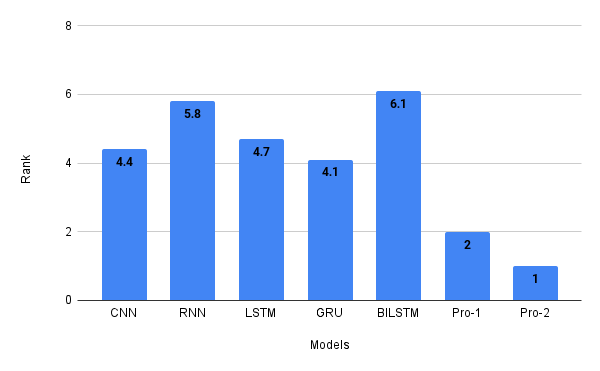
\includegraphics[scale=.7]{rankplot.png}
   \caption{Overall ranking of Traditional models \& Proposed models corresponding to all performance measures.}
 \end{figure*}

\begin{table}[htbp]
    \centering
    \caption{Non-parametric statistical analysis via Friedman ranking,  p-value \& Holm's procedure over various performance measure as RMSE,  MSE,  MAE and MAPE.}
    \begin{tabular}{cccccc}
        \toprule
        Error Metric & Models & RANK & P-value & Holm \\
        \midrule
        \multirow{5}{*}{RMSE} & CNN & 4.4 & \textbf{0.012827} & \textbf{0.016667} \\
        & RNN & 5.8 & \textbf{0.000443} & \textbf{0.01} \\
        & LSTM & 4.8 & \textbf{0.005414} & \textbf{0.0125} \\
        & GRU & 4 & \textbf{0.028108} & \textbf{0.025} \\
        & BiLSTM & 6 & \textbf{0.000253} & \textbf{0.008333} \\
        & Pro-1 & 2  & 0.464214 & 0.05\\
        & Pro-2 & \textbf{1}  & - & -\\
        \midrule
        \multirow{5}{*}{MSE} & CNN & 4.4 & \textbf{0.012827} & \textbf{0.016667} \\
        & RNN & 5.8 & \textbf{0.000443} & \textbf{0.01} \\
        & LSTM & 4.6 & \textbf{0.008415} & \textbf{0.0125} \\
        & GRU & 4 & \textbf{0.028108} & \textbf{0.025} \\
        & BiLSTM & 6.2 & \textbf{0.000141} & \textbf{0.008333} \\
        & Pro-1 & 2 & 0.464214 & 0.05 \\
        & Pro-2 & \textbf{1}  & - & -\\
        \midrule
        \multirow{5}{*}{MAE} & CNN & 5 & \textbf{0.003415} & \textbf{0.0125} \\
        & RNN & 5.4 & \textbf{0.00128} & \textbf{0.01} \\
        & LSTM & 4.4 & \textbf{0.012827} & \textbf{0.016667} \\
        & GRU & 4 & \textbf{0.028108} & \textbf{0.025} \\
        & BiLSTM & 6.2 & \textbf{0.000141} & \textbf{0.008333} \\
        & Pro-1 & 2 & 0.464214 & 0.05 \\
        & Pro-2 & \textbf{1}  & - & -\\
        \midrule
        \multirow{5}{*}{MAPE} & CNN & 3.4 & \textbf{0.078983} & \textbf{0.025} \\
        & RNN & 6.2 & \textbf{0.000141} & \textbf{0.008333} \\
        & LSTM & 5 & \textbf{0.003415} & \textbf{0.0125} \\
        & GRU & 4.4 & \textbf{0.012827} & \textbf{0.016667} \\
        & BiLSTM & 6 & \textbf{0.000253} & \textbf{0.01} \\
        & Pro-1 & 2 & 0.464214 & 0.05 \\
        & Pro-2 & \textbf{1}  & - & -\\
        \bottomrule
    \end{tabular}
    
    \label{tab:error_metrics}
\end{table}


 
 
 




























\section*{CRediT authorship contribution statement}

\textbf{S.Khan} : Conceptualization, methodology, formal analysis, Resource, Writing original draft, visualization.\\
\textbf{Vipin Kumar} : methodology, conceptualization, validation, investigation, writing, review editing, supervision.

\section*{Data availability}



The data is available on the Physionet website. A full clinical summary is included in the header (.hea) file of the majority of these ECG records, including age, gender, diagnosis, and, when appropriate, data on medical history, medicines and treatment, coronary artery pathology, ventriculography, echocardiography, and hemodynamics. The clinical summary for 22 individuals is unavailable. This database has shown to be a valuable research resource for ECG investigations.





\section*{Acknowledgments}

A heartfelt applause to the Physionet's attempt in making this research possible by providing free clinical records to study cardiovascular diseases by people who have no prior idea about clinical sciences. 

\label{}

% Numbered list
% Use the style of numbering in square brackets.
% If nothing is used,  default style will be taken.
%\begin{enumerate}[a)%\item 
%\item 
%\item 
%\end{enumerate}  

% Unnumbered list
%\begin{itemize}
%\item 
%\item 
%\item 
%\end{itemize}  

% Description list
%\begin{description}
%\item[]
%\item[] 
%\item[] 
%\end{description}  


\begin{comment}

\begin{table}[<options>]
\caption{}\label{tbl1}
\begin{tabular*}{\tblwidth}{@{}LL@{}}
\toprule
  &  \\ % Table header row
\midrule
 & \\
 & \\
 & \\
 & \\
\bottomrule
\end{tabular*}
\end{table}



\end{comment}
% Uncomment and use as the case may be
%\begin{theorem} 
%\end{theorem}

% Uncomment and use as the case may be
%\begin{lemma} 
%\end{lemma}

%% The Appendices part is started with the command \appendix;
%% appendix sections are then done as normal sections
%% \appendix




\label{}

% To print the credit authorship contribution details
\printcredits

%% Loading bibliography style file
%\bibliographystyle{model1-num-names}
\bibliographystyle{cas-model2-names}

% Loading bibliography database
\bibliography{ref}

% Biography
\bio{}
% Here goes the biography details.
\endbio

%\bio{pic1}
% Here goes the biography details.
\endbio

\end{document}

